%!TEX root =  Write_a_classifier.tex

%This section presents the datasets, the features, the experimental setting, evaluation methodology, and the experimental results.  %on Flower (102 classes)~\cite{Flower08} and CU-UCSD Bird Dataset (200 classes)~\cite{CU20010}.

\subsection{Datasets and Features}
\label{ss_ds_feats}
%\subsubsection{Datasets}
\noindent{\bf Datasets:}
We used  the CU200 Birds~\cite{CU20010} (200 classes - 6033 images) and the Oxford Flower-102~\cite{Flower08} (102 classes - ~8189 images) image dataset to test our methods, since they are among the largest and widely used fine-grained datasets.  We created  textual descriptions for each class in both datasets. The CUB200 Birds image dataset was created based on birds that have a corresponding Wikipedia article, so we have developed a tool to automatically extract Wikipedia articles given the class name. The tool succeeded to automatically generate 178 articles, and the remaining 22 articles was extracted manually from Wikipedia. These mismatches happens only when article title is a different synonym of the same bird class. On the other hand, Flower image dataset was not created using the same criteria as the Bird dataset, so classes of the Flower dataset classes does not necessarily have corresponding Wikipedia article. The tool managed to generate only 16 classes from Wikipedia out of 102, the remaining 86 articles was generated manually for each class from Wikipedia, Plant Database  \footnote{http://plants.usda.gov/java/}, Plant Encyclopedia \footnote{http://www.theplantencyclopedia.org/wiki/Main$\_$Page}, and BBC articles \footnote{http://www.bbc.co.uk/science/0/}. The collected textual description for FLower and Birds dataset are available here  \url{https://sites.google.com/site/mhelhoseiny/1202-Elhoseiny-sup.zip} .

\noindent{\bf Textual Feature Extraction:}
The textual features were extracted in two phases, which are typical in document retrieval literature. The first phase is an indexing phase that generates textual features with tf-idf (Term Frequency-Inverse Document Frequency) configuration (Term frequency as local weighting while inverse document frequency as a global weighting). The tf-idf is a measure of how important is a word to a text corpus. The tf-idf value increases proportionally to the number of times a word appears in the document, but is offset by the frequency of the word in the corpus, which helps to control for the fact that some words are generally more common than others. We used the normalized frequency of a term in the given textual description~\cite{salton1988term}. The inverse document frequency is a measure of whether the term is common; in this work we used the standard logarithmic idf~\cite{salton1988term}.   
The second phase is a dimensionality reduction step, in which  Clustered Latent Semantic Indexing (CLSI) algorithm~\cite{clsi05} is used. CLSI is a low-rank approximation approach for dimensionality reduction, used for document retrieval. In the Flower Dataset, tf-idf features $\in \mathbb{R}^{8875}$ and after CLSI the final textual features $\in \mathbb{R}^{102}$. In the Birds Dataset, tf-idf features is in $\mathbb{R}^{7086}$ and after CLSI the final textual features is in $\mathbb{R}^{200}$. 

\begin{comment}
\begin{table}
\scalebox(0.8){
\begin{tabular}{| c | c | c | c |}
\hline
\small
& \begin{minipage}[t]{0.22\columnwidth}%
tf-idf Features dimensions 
\end{minipage}  & \begin{minipage}[t]{0.17\columnwidth}CLSI Cluster count \end{minipage} & \begin{minipage}[t]{0.21\columnwidth}Reduced Dimensions \end{minipage}\\
\hline
\begin{minipage}[c]{0.17\columnwidth}Birds Dataset \end{minipage}&7086 & 200 & 200 \\
\hline 
\begin{minipage}[c]{0.17\columnwidth}Flower Dataset \end{minipage}&8875 & 102 & 102 \\
\hline
\end{tabular}}
\caption{Textual features specifications}
\label{clsiTextFsTable}
\end{table}

\end{comment}

%\subsubsection{Visual features}
\noindent{\bf  Visual features Extraction:}
We used the Classeme features~\cite{classemes} as the visual feature for our experiments since they provide an intermediate semantic representation of the input image. Classeme features are output of a set of classifiers corresponding to a set of $C$ category labels, which are drawn from an appropriate term list defined in~\cite{classemes}, and not related to our textual features. For each category $c \in \lbrace 1 \cdots C \rbrace $, a set of training images is gathered by issuing a query on the category label to an image search engine.
After a set of coarse feature descriptors (Pyramid HOG, GIST, \etc) is extracted, a subset of feature dimensions was selected~\cite{classemes}, and  a one-versus-all classifier $\varphi_{c}$ is trained for each category. The classifier output is real-valued, and is such that $\varphi_{c}(x) > \varphi_{c}(y)$ implies that $x$ is more similar to class $c$ than $y$ is. Given an image $x$,  the feature vector (descriptor) used to represent it is the classeme vector $  [\varphi_{1} (x),  \cdots, \varphi_{d_v} (x)]$, $d_v=2569$.

For Kernel classifier prediction, we evaluated  these features and also additional representations  for text descriptions (by the proposed distributional semantic kernel using word embedding) and  images ( (a) CNN features and (b)  combined kernel over different features learnt by MKL (multiple kernel learning)), discussed later in Subsection~\ref{ss_exp_kernel}.

%\subsubsection{Extracting Textual Features}
 

\begin{figure*}[ht!]
\centering
\hspace{-10mm}
\begin{minipage}{0.33\textwidth}
  \centering
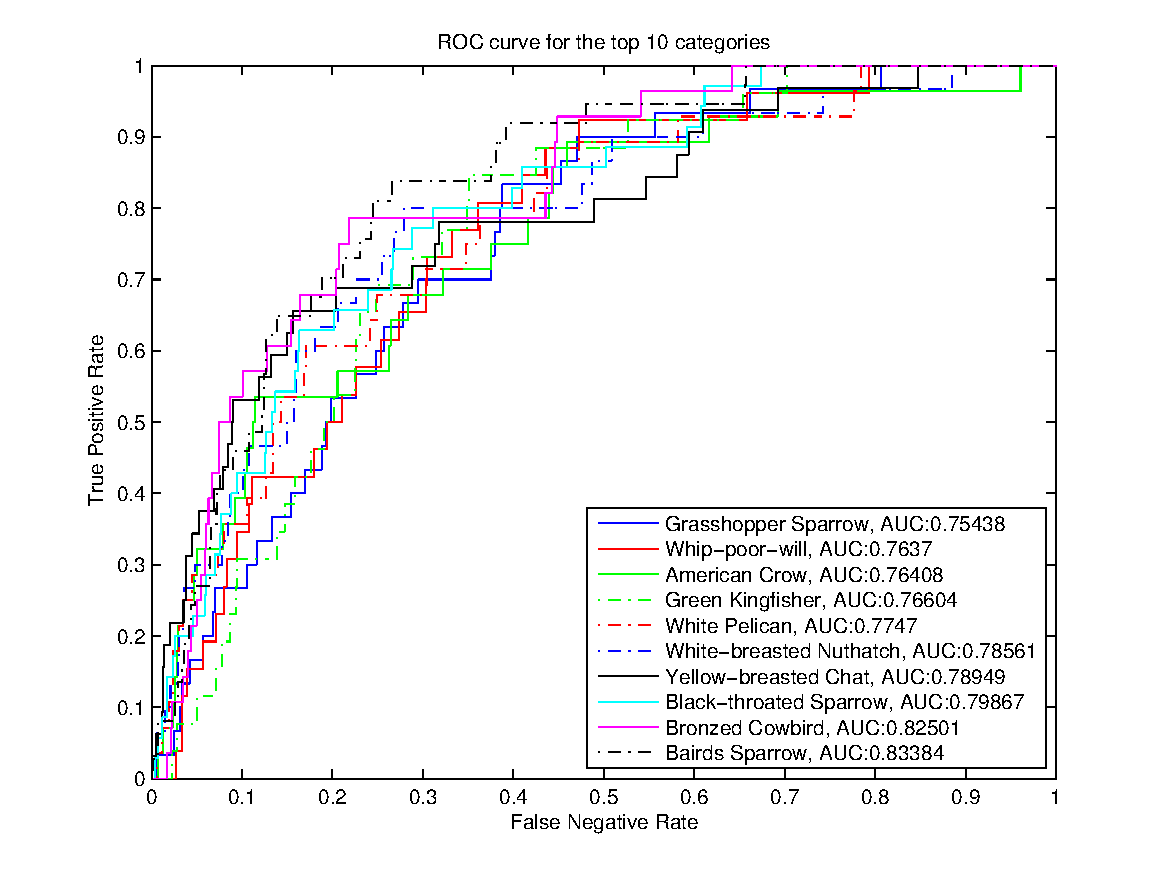
\includegraphics[width=1.1\linewidth,height=.75\linewidth]{birds_top10_ROC_final.eps}
%\vspace{-3mm}
\end{minipage}%
\hspace{-3mm}
\begin{minipage}{0.33\textwidth}
  \centering
 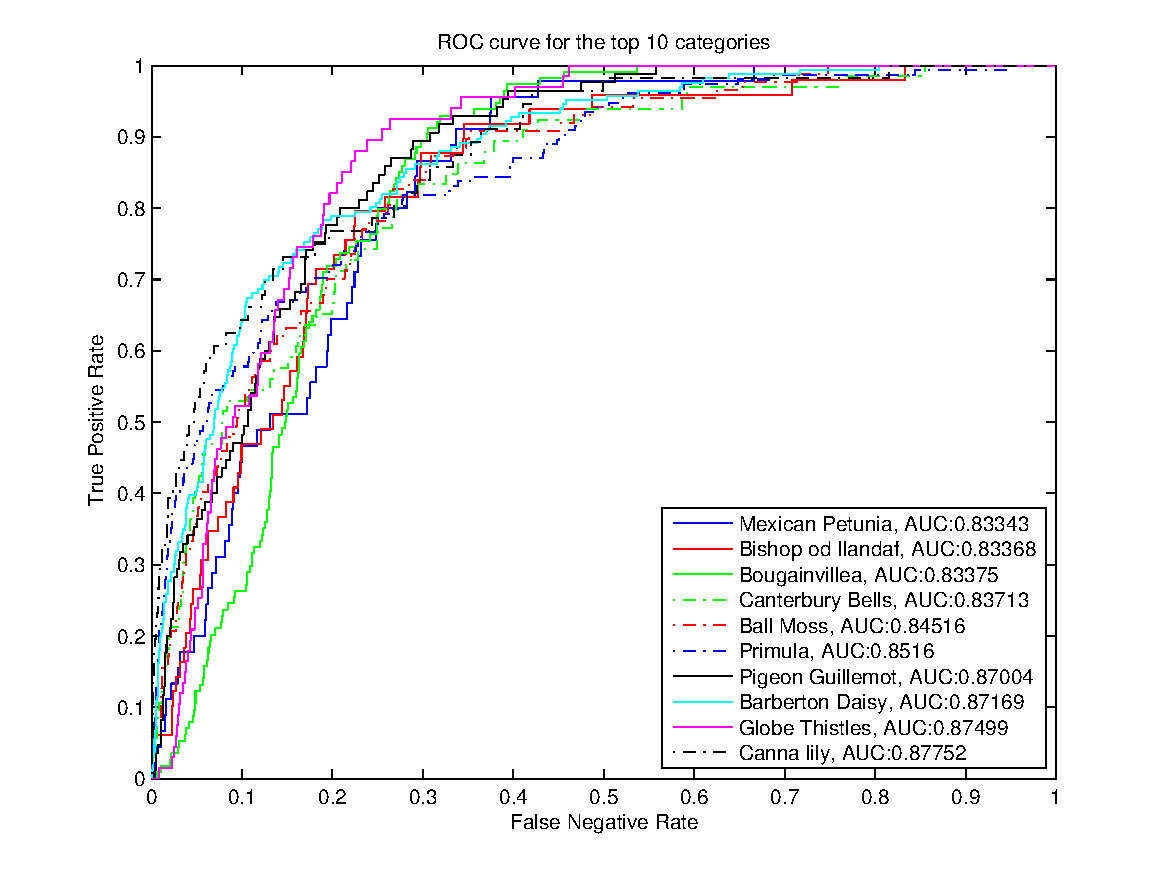
\includegraphics[width=1.1\linewidth,height=.75\linewidth]{flower_top10_ROC_final.eps}
 %\vspace{-3mm}
\end{minipage}
\begin{minipage}{0.33\textwidth}
  \centering
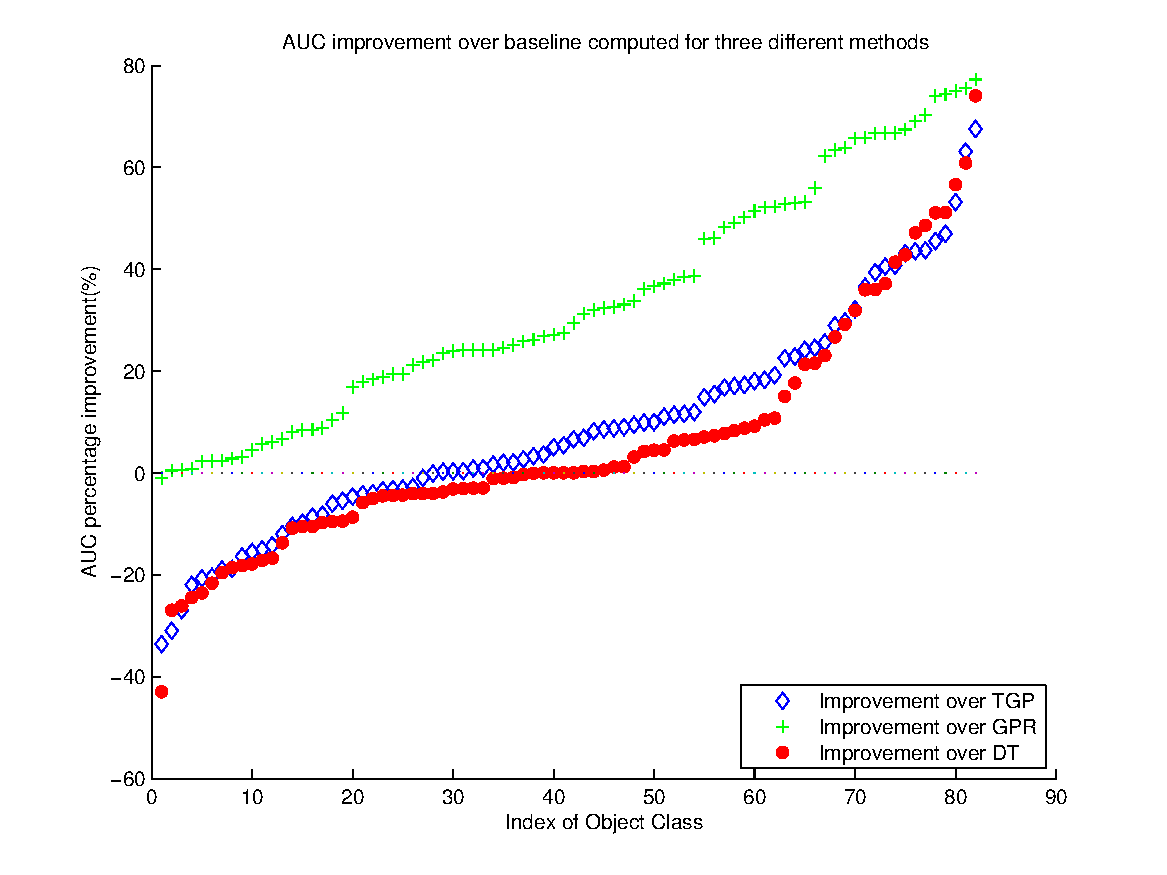
\includegraphics[width=1.1\linewidth,height=.75\linewidth]{flower_AUC_imp_final.eps}
%\vspace{-5mm}
\end{minipage}
\vspace{-1mm}
\caption{Linear : \textbf{Left and Middle}: ROC curves of best 10 predicted classes by the final formulation (E) for Bird  and Flower datasets respectively, \textbf{Right}: AUC improvement over the three baselines on Flower dataset (Formulations A (GPR), A (TGP), C). The improvement is sorted in an increasing order for each baseline separately (best seen in color)}
\vspace{-2mm}
\label{fig:result3fig}
\end{figure*}


\begin{table*}[b!]
\small
\centering
\caption{ Linear: Comparative Evaluation of Different Formulations on the Flower and Bird Datasets}
\label{T:AUC}
%\vspace{-10pt}
\scalebox{1.0}{
\begin{tabular}{|l|l|l|}
  \hline
  		&  Oxford Flowers   & UC-UCSD Birds   \\
  Approach  & Avg AUC (+/- std) & Avg AUC (+/- std)\\ 
  \hline
  \hline
  (A) Regression - GPR & 0.54 (+/- 0.02) & 0.52 (+/- 0.001) \\ 
  (A) Structured Regression - TGP & 0.58 (+/- 0.02) & 0.61 (+/- 0.02)\\
  (C)  Domain Transfer(DT) &  0.62(+/- 0.03)  &  0.59 (+/- 0.01)\\
  \hline 
  (B) Constrained GPR & 0.62(+/- 0.005) & - \\
  (B) Constrained TGP & 0.63(+/- 0.007) & - \\
  (D) Constrained Domain Adaptation (CDT) on Eq~\ref{eq:form} & 0.64 (+/- 0.006)& -  \\
       \hline
  (E) Regression+DT + constraints (final best linear approach) & {0.68} (+/- 0.01) & { 0.62} (+/- 0.02) \\
      \hline
\end{tabular}}
%\vspace{-10pt}
%\end{table}
%\begin{table}[t]
%\small
%\caption{\small Top-5 classes with highest combined improvement }
%\label{T:top5improv}
%\centering
%\vspace{-5pt}
\ignore{
{
\scalebox{0.7}{
\begin{tabular}{|l|l|l|l|l|}
  \hline
  \multicolumn{5}{c}{Top-5 Classes with highest combined improvement} \\
  \hline
  \hline
  class      &  (A) TGP (AUC) & (C) DT (AUC) & (D) TGP+DT+C  & \% Improv. \\
  \hline
  \hline
   2   &  0.51 & 0.55 & 0.83 & 57\% \\  
   28 & 0.52 & 0.54 & 0.76 &  43.5\% \\
   26 &  0.54 & 0.53 & 0.76 & 41.7\% \\
   81 & 0.52 & 0.82 & 0.87   & 37\%  \\
   37 & 0.72 & 0.53 & 0.83   & 35.7 \% \\
  \hline 
\end{tabular}}
}}
%\vspace{-5pt}
\end{table*}

\subsection{Experimental Results for Linear Classifier Prediction}


\noindent{\bf Evaluation Methodology:} Similar to zero-shot learning literature, we evaluated the performance of an unseen classifier in a one-vs-all setting where the test images of unseen classes are considered to be the positives and the test images from the seen classes are considered to be the negatives. We computed the ROC curve and report the area under that curve (AUC) as a comparative measure of different approaches. In zero-shot learning setting the test data from the seen class are typically very large compared to those from unseen classes. This makes other measures, such as accuracy, useless since high accuracy can be obtained even if all the unseen class test data are wrongly classified; hence we used ROC curves, which are independent of this problem. Five-fold cross validation over the classes were performed, where in each fold 4/5 of the classes are considered as ``seen classes'' and are used for training and 1/5th of the classes were considered as ``unseen classes'' where their classifiers are predicted and tested. Within each of these class-folds, the data of the seen classes are further split into training and test sets. The hyper-parameters for the  approach were selected through another five-fold cross validation within the class-folds  (i.e. the $80\%$ training classes are further split into $5$ folds to select the hyper-parameters). We made the seen-unseen folds used in our experiments available here \url{https://sites.google.com/site/mhelhoseiny/computer-vision-projects/Write_a_Classifier}.

\noindent{\bf Baselines:}
Since our work is the first to predict classifiers based on pure textual description, there are no other reported results to compare against. However, we designed three state-of-the-art baselines to compare against, which are designed to be inline with our argument in Sec~\ref{obvformulation}. Namely we used: 1) A Gaussian Process Regressor (GPR)~\cite{Rasmussen:2005}, 2) Twin Gaussian Process (TGP)~\cite{Bo:2010} as a structured regression method, 3)  Domain Transfer (DT)~\cite{da11}. The TGP and DT baselines are of particular importance since our formulation utilizes them, so we need to test if the formulation is making any improvement over them. It has to be noted that we also evaluate TGP and DT as alternative formulations that we are proposing for the problem, none of them was used in the same context before. %We  compared these baselines with formulations we proposed in section ~\ref{obvformulation} in including 4) Constrained GPR, 4) Constrained TGP, 5) Constrained DA, and 6) Constrained Regression  and Adaptation (our final approach).   

\begin{comment}
\begin{table}
\small
\centering
\caption{\small Comparative Evaluation on the Flowers and Birds}
\label{T:AUC}
%\vspace{-10pt}
\scalebox{1.0}{
\begin{tabular}{|l|l|l|}
  \hline
  		&  Flowers   & Birds   \\
  Approach  & Avg AUC (+/- std) & Avg AUC (+/- std)\\ 
  \hline
  \hline
  GPR  & 0.54 (+/- 0.02) & 0.52 (+/- 0.001) \\ 
  TGP  & 0.58 (+/- 0.02) & 0.61 (+/- 0.02)\\
  DT  &  0.62(+/- 0.03)  &  0.59 (+/- 0.01)\\
  Our Approach & {\bf 0.68} (+/- 0.01) & {\bf 0.62} (+/- 0.02) \\
  \hline 
\end{tabular}}
%\vspace{-10pt}
\end{table}

\end{comment}



\noindent{\bf Results:}
Table~\ref{T:AUC} shows the average AUCs for the final linear approach in comparison to the three baselines on both datasets. GPR performed poorly in all classes in both data sets, which was expected since it is not a structure prediction approach.  The DT formulation outperformed TGP in the flower dataset but slightly underperformed on the Bird dataset. The proposed approach outperformed all the baselines on both datasets, with significant difference on the flower dataset. It is also clear that the TGP performance was improved on the Bird dataset since it has more classes (more points are used for prediction). Fig ~\ref{fig:result3fig} shows the ROC curves for our approach on best predicted unseen classes from the Birds dataset on the Left  and Flower dataset on the middle. Fig ~\ref{F:AUCs} shows the AUC for all the classes on Flower dataset. %More results are attached in the supplementary materials. 
\begin{comment}
\begin{figure}
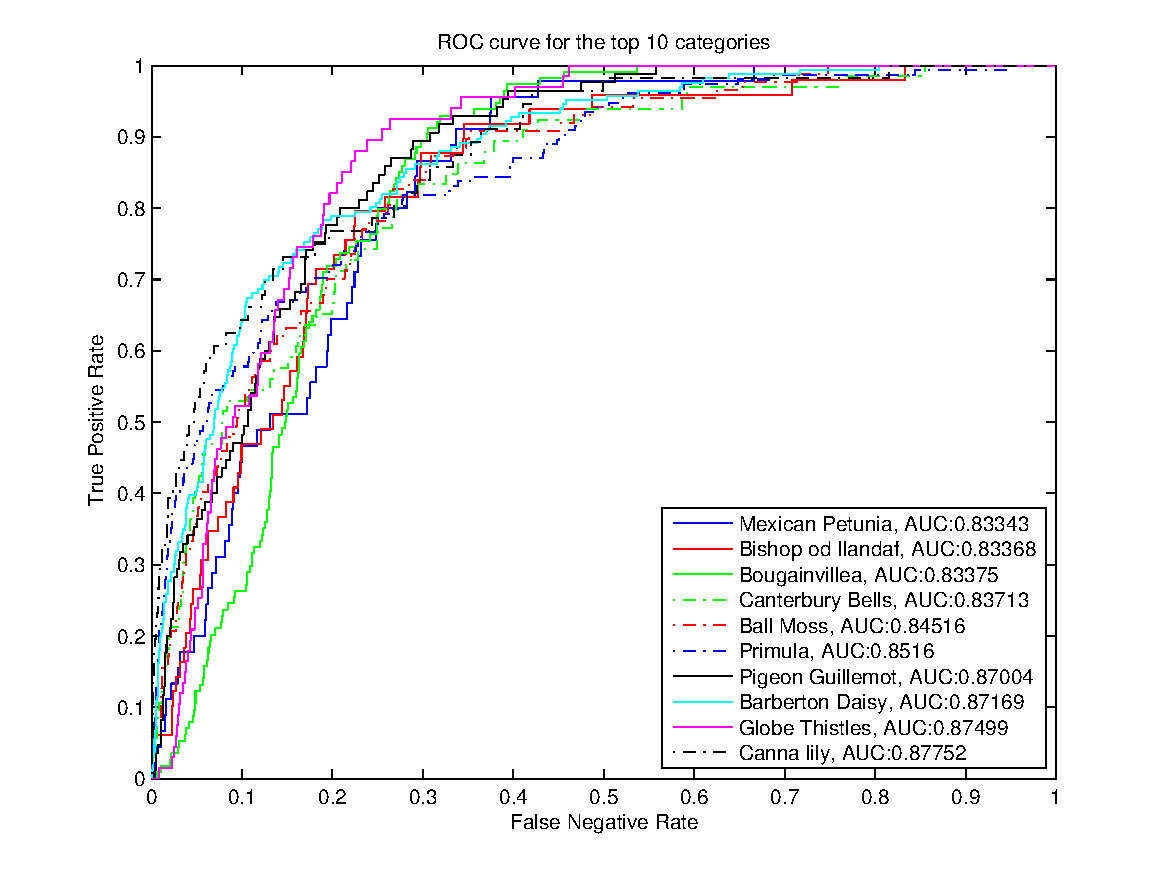
\includegraphics[width=0.9\linewidth,height=.6\linewidth]{flower_top10_ROC_final.eps}
%\vspace{-20pt}
\caption{ROC curves for best predicted classes -- Flower}
\label{F:bestROCs}
\end{figure}
\end{comment}
\begin{comment}
\begin{figure}
\centering
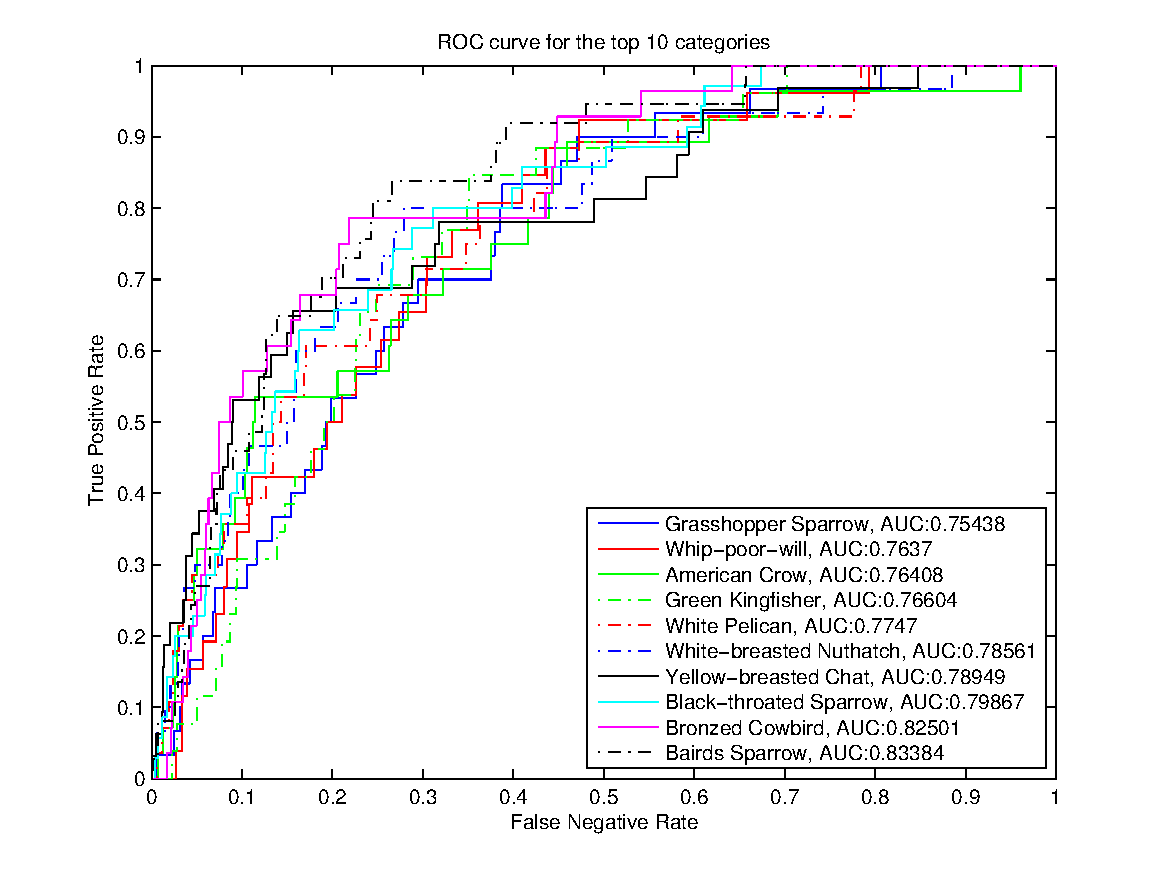
\includegraphics[width=0.8\linewidth,height=.5\linewidth]{birds_top10_ROC_final.eps}
%\vspace{-14pt}
\caption{ROC curves for best predicted classes -- Birds}
\label{F:bestROCsBIRDS}
%\vspace{-5pt}
\end{figure}
\end{comment}
\begin{comment}
\begin{figure}
\centering
\begin{minipage}{.45\textwidth}
  \centering
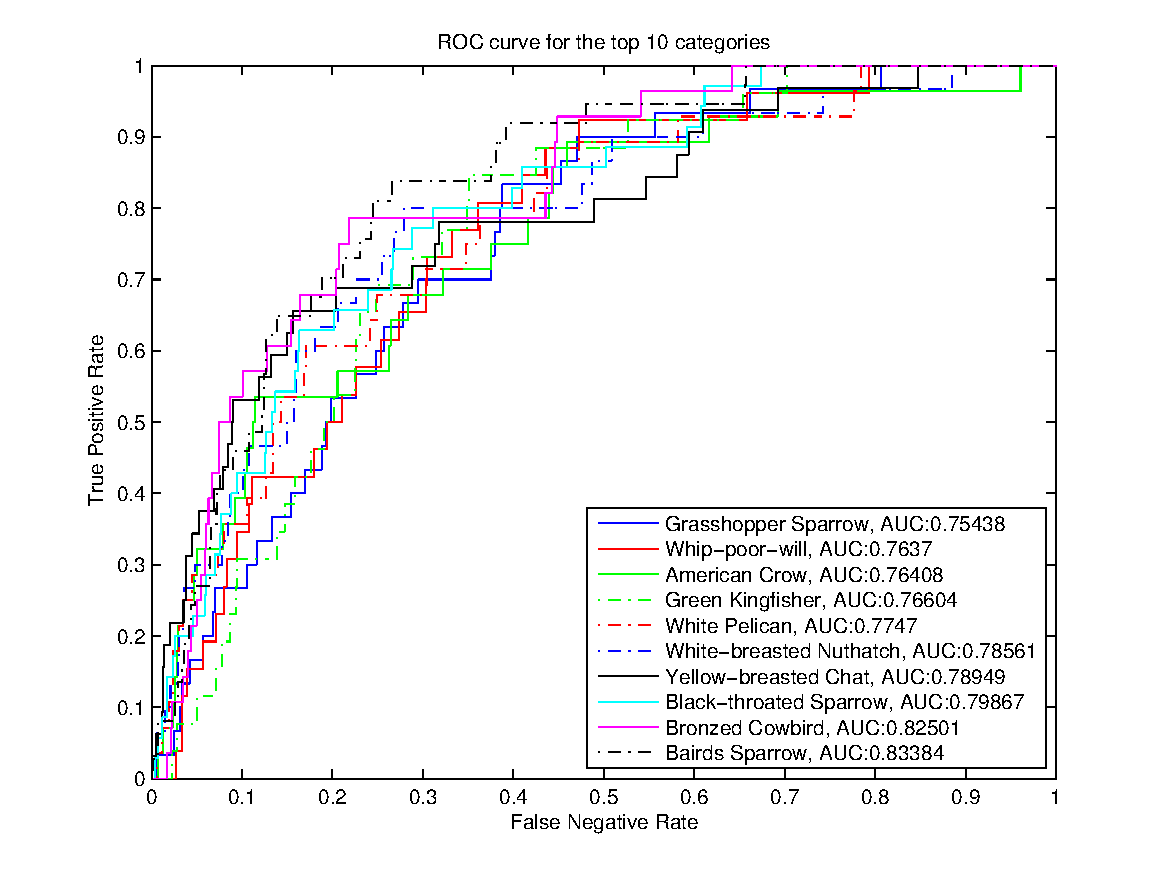
\includegraphics[width=0.43\linewidth,height=.4\linewidth]{birds_top10_ROC_final.eps}
	(a)
\end{minipage}%
\begin{minipage}{.45\textwidth}
  \centering
 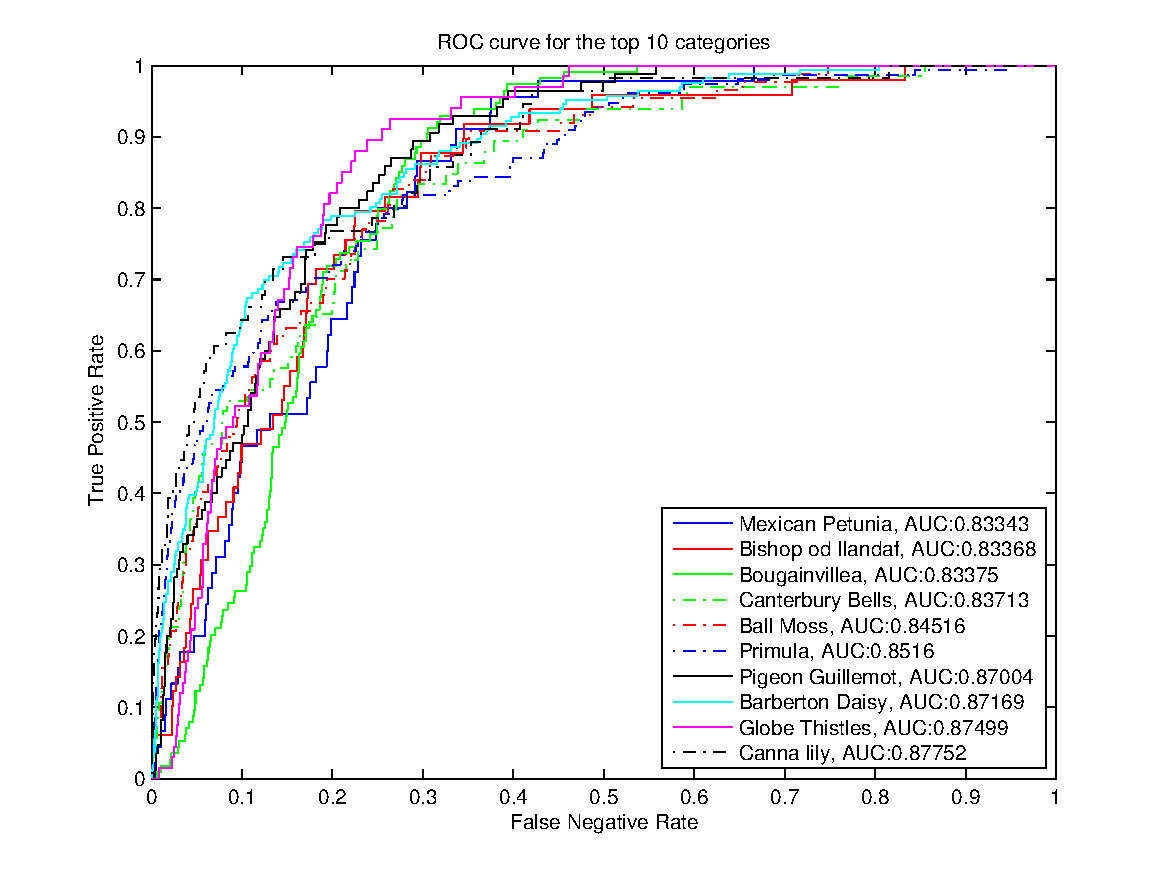
\includegraphics[width=0.43\linewidth,height=.4\linewidth]{flower_top10_ROC_final.eps}
 (b)
\end{minipage}
\end{figure}
\begin{figure}
        \begin{subfigure}[b]{0.45\textwidth}
                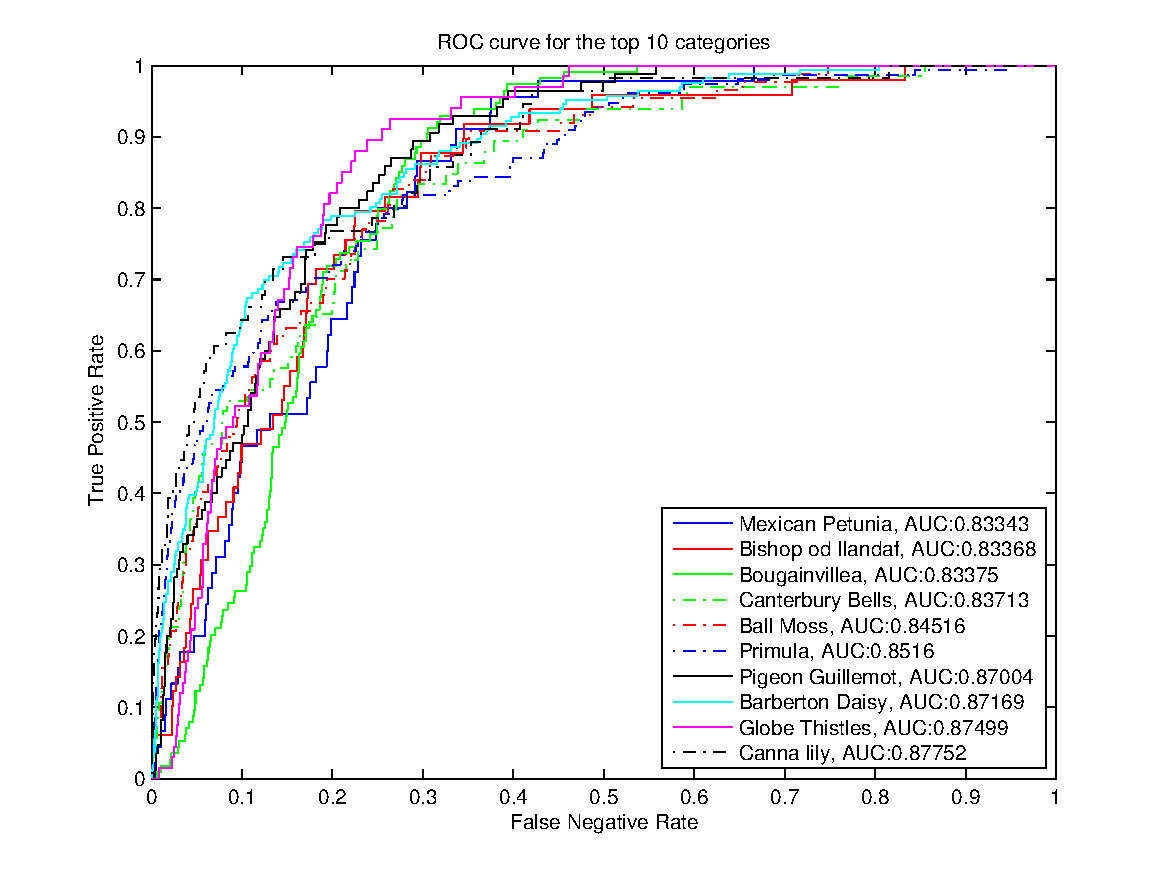
\includegraphics[width=0.4\linewidth,height=.4\linewidth]{flower_top10_ROC_final.eps}
                \caption{A gull}
                \label{fig:gull}
        \end{subfigure}\hspace{-20mm}
        \begin{subfigure}[b]{0.45\textwidth}
                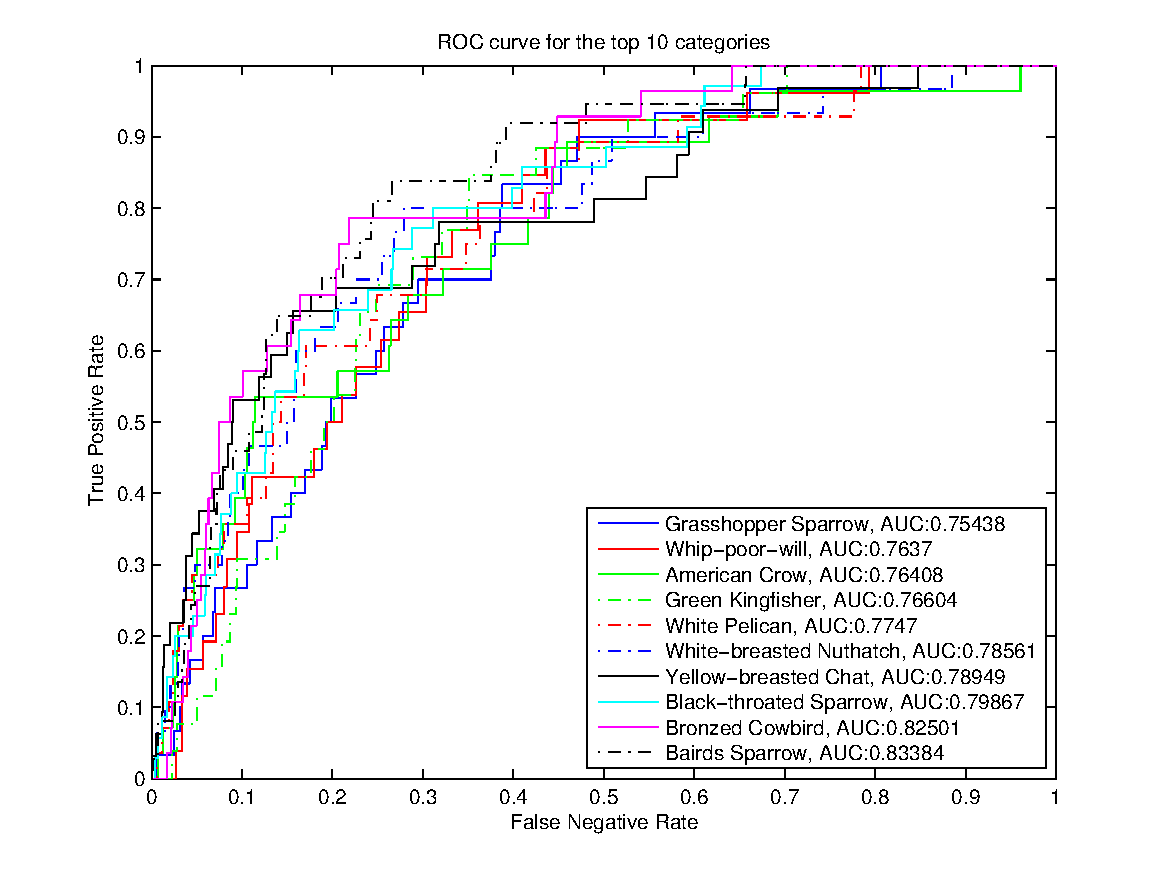
\includegraphics[width=0.4\linewidth,height=.4\linewidth]{birds_top10_ROC_final.eps}
                \caption{A tiger}
                \label{fig:tiger}
        \end{subfigure}
        \caption{Pictures of animals}
        \label{fig:animals}
\end{figure}
%\begin{center}
\end{comment}


%\end{center}



\begin{table}[t]
\small
\caption{\small Linear: Percentage of classes that the final proposed approach (formulation (E)) makes an improvement in predicting over the baselines (relative to the total number of classes in each dataset}
\label{T:classimprov}
%\vspace{-10pt}
\centering
\scalebox{1.0}{
\begin{tabular}{|l|l|l|}
  \hline
  		&  Flowers (102)  & Birds (200)\\ 
 baseline      &  \%  improvement & \%  improvement\\  
  \hline
  \hline
  (A) GPR  & 100 \% & 98.31 \% \\ 
  (A) TGP  & 66 \% & 51.81 \%\\
  (C) DT  &   54\% &  56.5\% \\
  %TGP+DA & 65\% &  55.45 \% \\
  \hline 
\end{tabular}}
%\vspace{-5pt}
\end{table}
\begin{comment}
\begin{figure}[t]
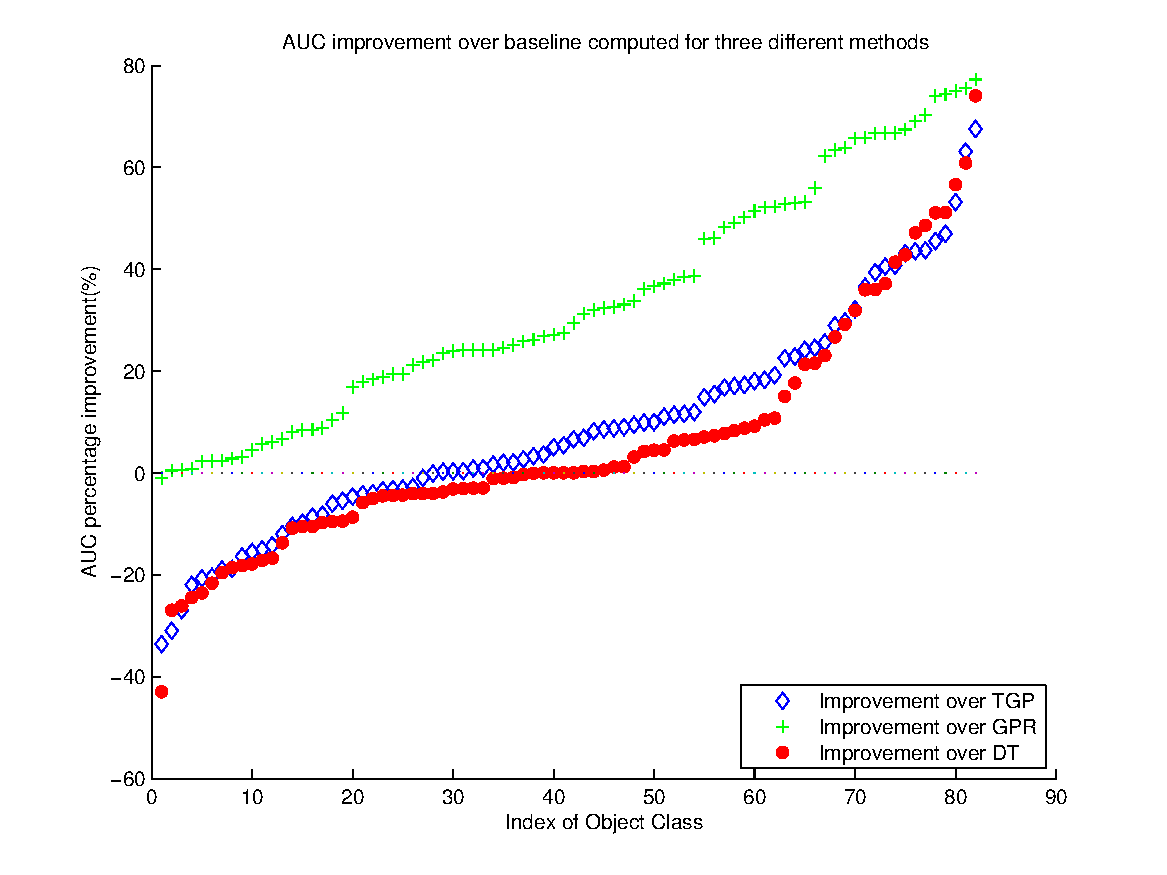
\includegraphics[width=0.95\linewidth,height=.5\linewidth]{flower_AUC_imp_final.eps}
%\vspace{-10pt}
\caption{AUC improvement over the three baselines. The improvement are sorted in a decreasing order for each baseline separately. }
\label{F:AUC_improvement}
\end{figure}
\end{comment}
Fig ~\ref{fig:result3fig}, on the right, shows the improvement over (A) GPR,\begin{figure}
\vspace{-3mm}
\centering
 \hspace*{-12mm}%
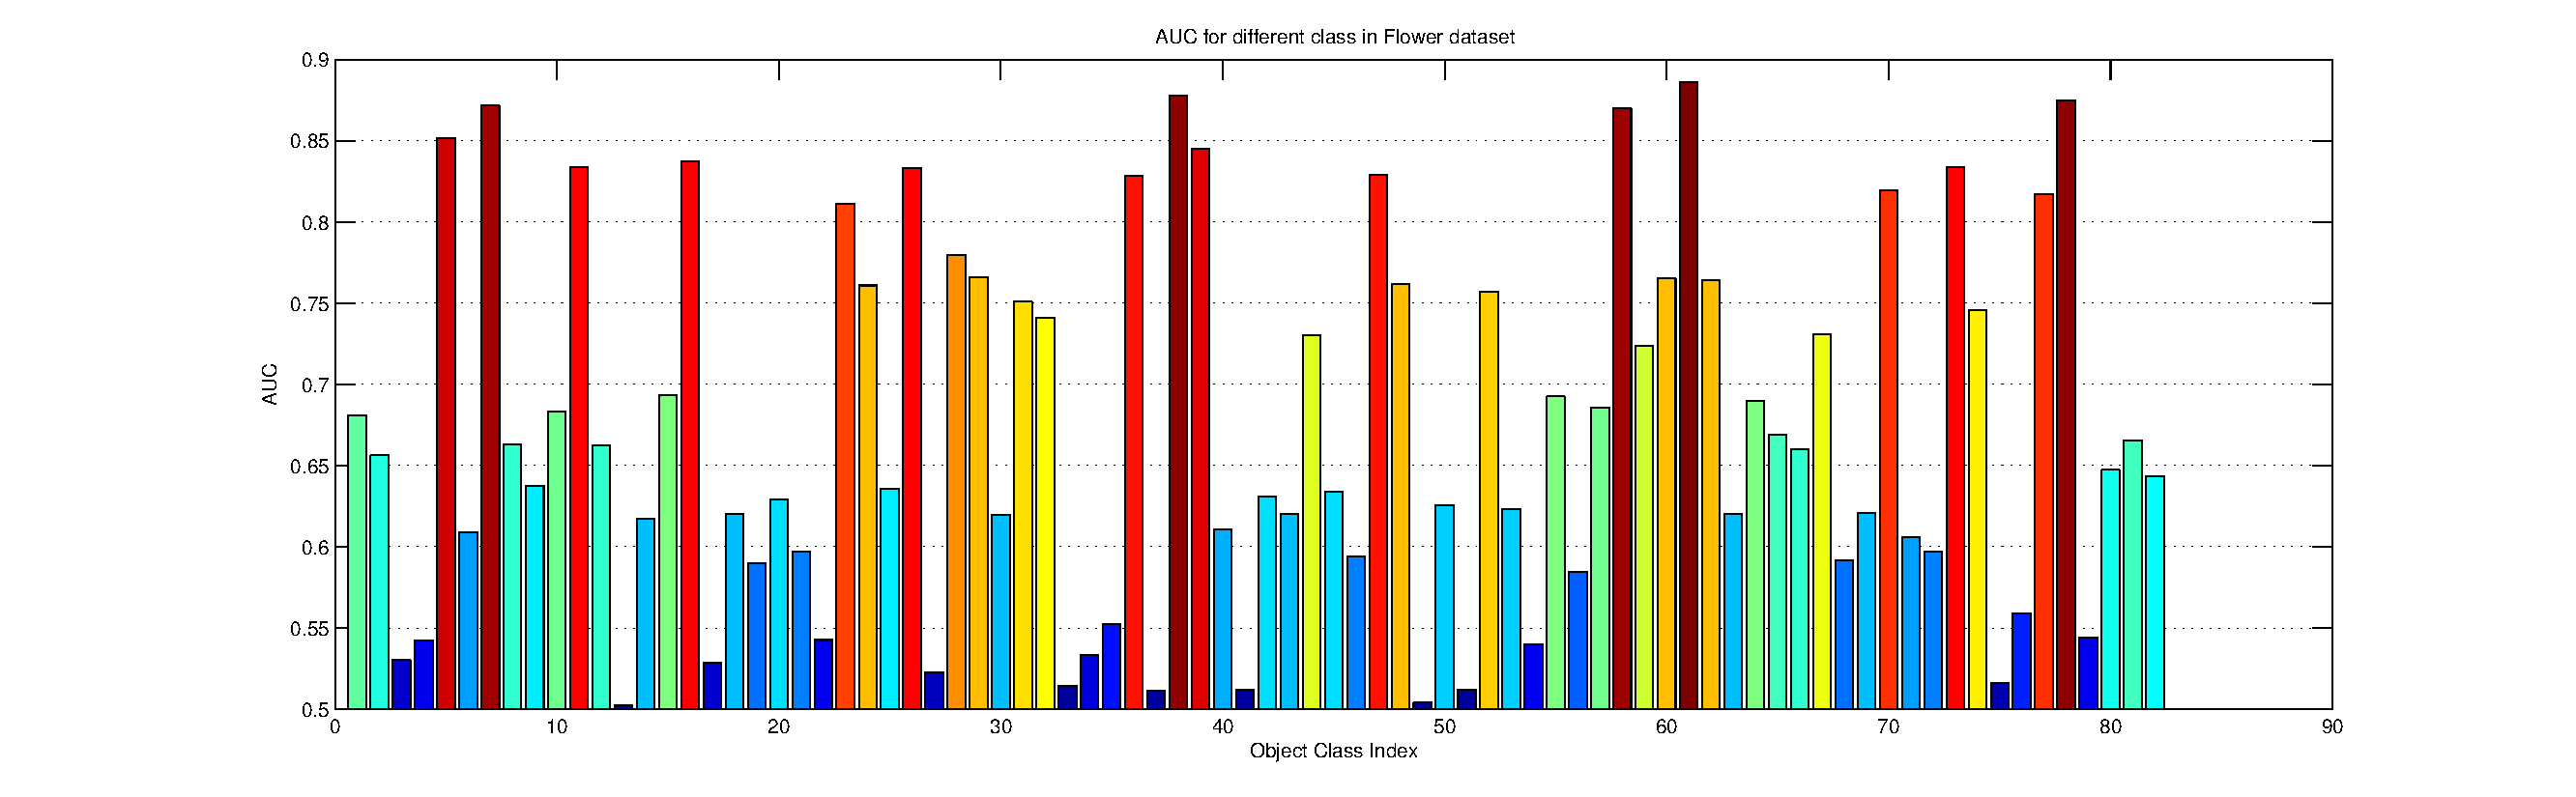
\includegraphics[width=1.24\linewidth,height=.27\linewidth]{flower_AUC_for_all_classes_final.eps}
%\vspace{-15pt}
\caption{Linear: AUC of the predicated classifiers for all classes of the flower datasets (Formulation E)}
\label{F:AUCs}
\end{figure} A(TGP), and (C) DT for each class, where the improvement is calculated as (our AUC- baseline AUC)/ baseline AUC \%. 
Table~\ref{T:classimprov} shows the percentage of the classes which our approach makes a prediction improvement for each of  the three baselines\begin{comment}. The last row show the improvement over both the TGP and DT baseline 
\end{comment}
. Table~\ref{T:top5improv} shows the five classes in Flower dataset where our approach made the best average improvement.
\begin{comment}. (TGP+DT).  
\end{comment}
 The point of that table is to show that in these cases both TGP and DT did poorly while our formulation that is based on both of them did significantly better. This shows that our formulation does not simply combine the best of the two approaches but can significantly improve the prediction performance.

\begin{table}[t]
\small
\caption{\small Linear: Top-5 classes with highest combined improvement in Flower dataset}
\label{T:top5improv}
\centering
%\vspace{-5pt}
{
\scalebox{0.85}{
\begin{tabular}{|l|l|l|l|l|}
  \hline
  class      &  (A) TGP (AUC) & (C) DT (AUC) & (E) Our (AUC)  & \% Improv. \\
  \hline
  \hline
   2   &  0.51 & 0.55 & 0.83 & 57\% \\  
   28 & 0.52 & 0.54 & 0.76 &  43.5\% \\
   26 &  0.54 & 0.53 & 0.76 & 41.7\% \\
   81 & 0.52 & 0.82 & 0.87   & 37\%  \\
   37 & 0.72 & 0.53 & 0.83   & 35.7 \% \\
  \hline 
\end{tabular}}
}
\vspace{-2pt}
\end{table}







To evaluate the effect of the constraints in the objective function, we removed the constraints $- (\mathbf{c}^\textsf{T} {\mathbf{x}}_{i} ) \geq \zeta_i$ which try to enforces all the seen examples to be on the negative side of the predicted classifier hyperplane and evaluated the approach. The result on the flower dataset (using one fold) was reduced to average AUC=0.59 compared to AUC=0.65 with the constraints. Similarly, we evaluated the effect of the constraint  $\mathbf{t}_*^\textsf{T} \mathbf{W} \mathbf{c} \ge l$. The result was reduced to average AUC=0.58 compared to AUC=0.65 with the constraint.  This illustrates the importance of this constraint in the formulation.

\noindent{\bf Constrained Baselines:}
%\textbf{different formulations experiments:}
\ignore{We computed the ROC curves and report the area under that curve (AUC) as a comparative measure\footnote{In zero-shot learning setting the test data from the seen class are typically very large compared to those from unseen classes. This makes other measures, such as accuracy, useless since high accuracy can be obtained even if all the unseen class test data are wrongly classified; hence we used ROC curves, which are independent of this problem.} Five-fold cross validation over the classes were performed, within each of these class-folds, the data of the seen classes are further split into training and test sets.}
Table~\ref{T:AUC} (bottom three lines) also shows the average AUCs for the constrained baselines formulations, namely Constrained GPR, TGP and DT; see section~\ref{formulation}. Even though the visual features and textual features were independently extracted, by learning correlation between them, we can predict classifiers for new categories. As shown previously, GPR performed poorly, while, as expected, TGP performed better. Adding constraints to GPR/TGP improved their performance. Combining regression and DT gave significantly better results for classes where both approaches individually perform poorly, as can be seen in Table~\ref{T:AUC}-right. We performed an additional experiment, where  $\mathbf{W}$ is firstly computed using Constrained Domain Transfer (CDT). Then, the unseen classifier is predicted using equation~\ref{eq:form} with $\gamma=0$, which performs worse. This indicates that adding constraints to align to seen classifiers hurts the learnt domain transfer function on unseen classes. In conclusion, the final formulation that combines TGP and DT with additional constraints performs the best in both Birds and Flower datasets, where the effect of TGP is very limited since it was trained on sparse points. 

%\begin{float}





\subsection{Experimental Results for Kernel Classifier Prediction}
\label{ss_exp_kernel}


%!TEX root = ZeroShotLearningECCV14.tex
\ignore{
Now that we have described our zero-shot learning setting and the suggested approaches to directly predict kernel-classifier parameters for unseen classes, we present several experiments to validate our model.
}
\ignore{In this section, we presented a set of experiments, conducted to evaluate our proposed model for zero-shot learning of visual classifiers. The quantitative comparisons show our superior performance to the state of the art on two challenging datasets of fine-grained object categories.}
%\subsection{Datasets}


%We performed three experiments to validate our model on two challenging fine-grained recognition datasets. Two of experiments were performed on UCSD-Birds dataset \cite{CU20010}, while the remaining one was performed on Oxford-Flower dataset \cite{Flower08}. UCSD-Birds dataset consists of 200 classes, total of 6033 images. On the other hand, the Flower dataset consists of 102 flower categories, and total of 8189 images. For the first two experiments, we used the textual descriptions' augmentation provided by  for Birds and Flower datasets,  as privileged information provided for each class description. In the third experiment, we used the average attribute vector of each class in Birds dataset as privileged information. Unlike typical attribute-based approaches, that learn attribute classifiers as an intermediate representation, our approach does not need to learn any attribute classifiers. Next subsections details the experimental settings and the features.

\subsubsection{Additional Evaluation Metrics}

In addition to the the AUC, we already studied in the previous section. We report two additional metrics while evaluating and comparing the kernel classifier prediction to the linear classifier prediction, detailed as follows. 

%\textit{AUC:}  In order to measure the discriminative ability of our predicted one-vs-all classifier for each unseen class, against the seen classes, we report the area under the ROC curve. \ignore{This is because a large accuracy could be achieved even if all unseen points are incorrectly classified.} Since unseen class positive examples are few compared to negative examples, a large accuracy could be achieved even if all unseen points are incorrectly classified. Hence, AUC is a more consistent measure, compared to accuracy for this purpose.  In this setting, we use the predicted classifier of an unseen class as a binary separator against the seen classes. This measure is computed for each predicted unseen classifier and the average AUC is reported as well. This is the only measure addressed in \cite{Hoseini13} to evaluate the unseen classifiers, which is limiting in our opinion. Instead, we cover the following additional metrics to evaluate explicit classifier prediction. 

\textit{\small$|N_{sc}|\,$\normalsize to \small$|N_{sc}+1|\,$\normalsize Recall:}
Under this metric, we aim to check  how   the learned classifiers of the seen classes confuse the predicted classifiers, when they are involved in a multi-class classification problem of \small$N_{sc} + 1\,$\normalsize classes. \ignore{The first \small$N_{sc}\,$\normalsize classifiers are those of the seen classes, while \small$({N_{sc}+1})^{st}$\normalsize classifier is a predicted classifier for an unseen class. }We use Eq~\ref{eq:mclass} to predict label $l^*$  with the maximum confidence of an image \small$x^*$\normalsize, such that \small$l^* \in {L}_{sc} \cup l_{us}$\normalsize,  \small$l_{us}\,$\normalsize is the label of the ground truth unseen class, and ${L}_{sc}$ is the set of seen class labels. We compute the recall under this setting. This metric is computed for each predicted unseen classifier and the average is reported.

\textit{Multiclass Accuracy of Unseen classes (MAU):} Under this setting, we aim to evaluate the performance of  the unseen  classifiers against each others. Firstly, the classifiers of all unseen categories are predicted. Then, we use Eq~\ref{eq:mclass} to predict the label with the maximum confidence of a test image $x$, such that its label $l_{us}^* \in {L}_{us}$, where ${L}_{us}$ is the set of all unseen class labels that only have text descriptions. 



%Table~\ref{tab:settings} shows the settings of the three experiments, we performed on Flower and Birds datasets, where $|{Y}_{sc}|$ and $|{Y}_{us}|$ are the number of the seen and the unseen classes, respectively. In these experiments $\mathcal{D}_{train} =\{ \mathcal{S}_x = \{(\textbf{x}_i,y_i)\}_N , \mathcal{S}_e = \{ y_i, \textbf{e}_i\}_{N_{sc}} \}$ involves $80\%$ of the classes in the dataset, and $D_{test} = \{ \mathcal{S}_x^*= \{ \textbf{x}^*_j \}_{N'}, \mathcal{S}_e^* = \{ y^*_j, \textbf{e}_{y^*_j} \}_{N_{us}} \}$ involves $20\%$ of the classes in the dataset. This data split is applied for both Birds and Flower datasets, as illustrated in Table ~\ref{tab:settings}.

%\begin{table}[h!]
%\caption{The experimental settings}
%\label{tab:settings}
%\centering
%\begin{tabular}{|c|c|c|c|c|c|}
%\hline 
% & Dataset & $\mathcal{E}$ domain & $\mathcal{X}$ domain & $|\mathcal{Y}_{sc}|$ & $|\mathcal{Y}_{us}|$ \\ 
%\hline 
%Expr 1 & Flower & text  & classeme & 80 & 22 \\ 
%\hline 
%Expr 2 & Birds & attributes & classeme & 160 & 40 \\ 
%\hline 
%Expr 3 & Birds & text & classeme & 160 & 40 \\ 
%\hline 
%\end{tabular} 
%\end{table}




\subsubsection{Comparisons to Linear Classifier Prediction}
\label{exp1}
 We compare the kernel methods to the linear prediction discussed earlier,  which predicts a linear classifier from textual descriptions  ( \small$\mathcal{T}\,$\normalsize space in our framework). The aspects of the comparison includes  1) whether the predicted kernelized classifier outperforms the predicted linear classifier  2) whether this behavior is consistent on multiple datasets. We performed the comparison on both Birds and Flower dataset.  For these experiments, in our setting, domain \small$\mathcal{V}\,$\normalsize is the visual domain and domain \small$\mathcal{T}\,$\normalsize is the textual domain, \ie, the goal is to predict classifiers from pure textual description. We used the same features on the visual domain  and the textual domains detailed in subsection~\ref{ss_ds_feats}. That is,  classeme features \cite{classemes} for images, extracted from images of the Bird and the Flower datasets and tf-idf~\cite{salton1988term} features for text articles followed by a CLSI~\cite{clsi05} dimensionality reduction phase. %Classeme  is a 2569-dimensional features, which correspond to confidences of a set of one-vs-all classifiers, pre-trained on images from the web, as explained in~\cite{classemes}, not related to either the Bird nor the Flower datasets. The rationale behind using these features in~\cite{Hoseini13} was that they offer a semantic representation\ignore{ represent semantic-level features, which would have better chance in correlating with the textual features}.
  %For the textual domain, we used the same textual feature extracted by~\cite{Hoseini13}. In that work, 
 %tf-idf (Term-Frequency Inverted Document Frequency)\cite{salton1988term} features were extracted from the textual articles were used, followed by a CLSI~\cite{clsi05} dimensionality reduction phase.
 
We denote our kernel Domain Transfer prediction  and one class SVM adjust DT prediction by  ``DT-kernel'' and ``SVM-DT-kernel'' respectively. We compared against  linear classifier prediction (Linear Formulation (E) approach, denoted by just Linear Classifier).  \ignore{(which uses a quadratic program to optimize the classifier parameters)}We also compared against the  linear direct domain transfer (Linear Formulation (C), denoted by DT-linear).  In our kernel approaches, we used Gaussian rbf-kernel as a similarity measure in \small$\mathcal{T}\,$\normalsize and \small$\mathcal{V}\,$\normalsize spaces (\ie \small$k(d,d') = exp(-\lambda ||d-d'||)$\normalsize). 

 
%\textbf{Text features as $\mathcal{E}$  (Expr1 [Flower], Expr2 [Birds] )}
%We start by presenting AUC an MAU metrics on Flower and Birds dataset, we follow that by an argument on  the results.
\begin{table*}[hb!]
\vspace{-1mm}
 \begin{minipage}{0.56\linewidth}
\caption{Kernel: Recall, MAU, and average AUC on three seen/unseen splits on Flower Dataset and a seen/unseen split on Birds dataset}
\label{tbl:flowerbirdsmauauc}
  \centering
  \scalebox{0.90}
  {
\begin{tabular}{|c|c|c|c|c|}
\hline 
  & \textbf{Recall-Flower} & improvement & \textbf{Recall-Birds}& improvement \\ 
  \hline 
{SVM-DT kernel-rbf }& \textbf{40.34\% (+/-  1.2) \%} & & \textbf{44.05 \%}   &  \\ 
\hline 
Linear Classifier  & 31.33  (+/-  2.22)\% & 27.8 \%  & 36.56 \% & 20.4 \% \\ 
\hline 
\end{tabular}}

\hspace{-1.5mm}\scalebox{0.943}
  {
\begin{tabular}{|c|c|c|c|c|}
\hline 
  & \textbf{MAU-Flower} & improvement & \textbf{MAU-Birds}& improvement \\ 
  \hline 
{SVM-DT kernel-rbf }& \textbf{9.1 (+/-  2.77) \%} & & \textbf{3.4  \%}   &  \\ 
\hline 
{DT kernel-rbf }& \textbf{6.64 (+/-  4.1) \%} & 37.93 \%  & \textbf{2.95  \%} & 15.25 \% \\ 
\hline 
Linear Classifier \ignore{ Prediction} & 5.93  (+/-  1.48)\% & 54.36 \%  & 2.62 \% & 29.77 \% \\ 
\hline 
DT-linear\ignore{~\cite{Hoseini13,da11}} & 5.79 (+/-  2.59)\% & 58.46 \%  &  2.47 \% & 37.65 \%  \\ 
\hline 
\end{tabular}}
\scalebox{0.93}
  {
\begin{tabular}{|c|c|c|c|c|} 
\hline 
 & \textbf{AUC-Flower}& improvement & \textbf{AUC-Birds} & improvement\\ 
\hline 
{SVM-DT kernel-rbf }& {0.653 (+/-  0.009) } &   &   0.61  &   \\ 
\hline 
{DT kernel-rbf }& {0.623 (+/-  0.01) \%} & 4.7 \% &  0.57  & 7.02 \%  \\ 
\hline 
Linear Classifier \ignore{Prediction} & 0.658 (+/-  0.034) & - 0.7 \% & 0.62  & -1.61\%  \\ 
\hline 
Domain Transfer\ignore{~\cite{Hoseini13,da11}} &0.644 (+/-  0.008) &  1.28 \% & 0.56  & 8.93\%  \\ 
\hline 
\end{tabular} 
}
%\vspace{-5mm}
\end{minipage}
 \begin{minipage}{00.02\linewidth}
 $\,\,$
 \end{minipage}
\begin{minipage}{0.42\linewidth}
\centering
   \caption{Kernel: MAU on a seen-unseen split-Birds Dataset (MKL)}
\label{tbl:birdsmkl}
 \scalebox{0.93}
  {
\begin{tabular}{|c|c|c|}
\hline 
& MAU & improvement \\ 
\hline 
{SVM-DT kernel-rbf (text)}& \textbf{4.10  \%} &   \\ 
\hline 
Linear Classifier \ignore{Prediction} & 2.74 \% & 49.6 \% \\ 
\hline 
\end{tabular} }

\centering
     \vspace{5mm}
   \caption{Kernel: MAU on a seen-unseen split-Birds Dataset (CNN image features, text description)}
     %\vspace{-1mm}
\label{tbl:birdscnn}
 \scalebox{0.93}
  {
\begin{tabular}{|c|c|c|}
\hline 
& MAU & improvement \\ 
\hline 
\hline 
{SVM-DT kernel ($\mathcal{V}$-rbf, $\mathcal{T}$-DS kernel)}& \textbf{5.35  \%} &   \\ 
\hline
{SVM-DT kernel ($\mathcal{V}$-rbf, $\mathcal{T}$-rbf on TFIDF)}& \textbf{4.20  \%} &  27.3\% \\ 
\hline 
Linear Classifier (TFIDF text) \ignore{Prediction} & 2.65 \% & 102.0\% \\ 
\hline 
\cite{norouzi2014zero} & 2.3\% & 132.6\% \\
\hline 
\end{tabular} }
 %\vspace{-5mm}
\end{minipage}
\vspace{-4mm}
\end{table*}




\textit{Recall metric : } The recall of the SVM-DT kernel approach is 44.05\% for Birds and 40.34\% for Flower, while it is 36.56\% for Birds and  31.33\% for Flower by best Linear Classifier prediction (E). This indicates that the  predicted classifier is less confused by the classifiers of the seen compared with  Linear Classifier prediction; see table ~\ref{tbl:flowerbirdsmauauc} (top part)


\textit{MAU metric:} It is worth to mention that the multiclass accuracy for the trained seen classifiers is $51.3\%$ and $15.4\%$, using the classeme features,  on Flower dataset and Birds dataset\footnote{Birds dataset is known to be a challenging dataset for fine-grained, even when applied in a regular multiclass setting as it is clear from the $15.4\%$ performance on seen classes}, respectively. Table ~\ref{tbl:flowerbirdsmauauc} (middle part) shows the average $MAU$ metric over three seen/unseen splits for Flower dataset and one split on Birds dataset, respectively. 
Furthermore, the relative improvements of our  SVM-DT-kernel approach is reported against the baselines. On Flower dataset,  it is interesting to see that our approach achieved $9.1\%$ MAU, $182\%$ the random guess performance, \ignore{, which is $17.7\%$ of the multi-class accuracy of the seen classes (i.e. $51.3\%$),} %\footnote{$17.7 = 9.1 / 51.3 \cdot 100$}
by predicting the unseen classifiers using just textual features as privileged information (i.e. $\mathcal{T}$ domain). It is important to mention that we achieved also $13.4\%$, $268\%$ the random guess performance, in one of the splits (the 9.1\% is the average over 3 seen/unseen splits). Similarity on Birds dataset, we achieved $3.4\%$ MAU from text features, $132\%$  the random guess performance (further improved up to $224\%$ in next experiments).\ignore{, which is $22.7\%$ of the multi-class accuracy of the seen classes on the same dataset ($15.4\%$)}


\textit{AUC metric: } Fig\ignore{~\ref{F:top10} }~\ref{F:AUCstop10} (top part) shows the ROC curves for our approach on the best predicted unseen classes from the Flower dataset. Fig\ignore{~\ref{F:AUCs}}~\ref{F:AUCstop10} (bottom part) shows the AUC for all the classes on Flower dataset (over three different splits). Table~\ref{tbl:flowerbirdsmauauc} (bottom part)  shows the average AUC on the two datasets, compared to the baselines. More results and figures \ignore{Corresponding figures for Birds dataset } for our kernel approach are attached in the supplementary materials.

Looking at table~\ref{tbl:flowerbirdsmauauc}, we can notice that the proposed approach performs marginally similar to the baselines from AUC perspective. However, there is a clear improvement  in MAU  and Recall metrics. These results show the advantage of predicting classifiers in kernel space. Furthermore, the table shows that our SVM-DT-kernel approach outperforms our DT-kernel model. This indicates the advantage of the class separation, which is adjusted by the SVM-DT-kernel model. \ignore{In all these experiments, we used a setting of our SVM-DT-kernel model, where \small$C_{\beta}({ \textbf{T}} )\,$\normalsize is ignored (i.e. \small$\lambda_2 = 0$\normalsize)\ignore{; see Sec ~\ref{ss:tr}}). In order to study whether \small$C_{\beta}( \textbf{T} )\,$\normalsize is effective in unseen class prediction, we performed an extra experiment on Birds dataset, where \small$\lambda_2>0\,$\normalsize (e.g. \small$\lambda_2 =1$\normalsize). We found that MAU of our DT approach has slightly decreased (i.e from $2.95\&$  to $2.91\%$ ). Under the same setting, we also found that  \small$C_{\beta}( \textbf{T} )\,$\normalsize  slightly reduced the performance of SVM-DT from $9.1\%$ to $8.98\%$.MAU. This reflect our intuition argued in the approach section\ignore{Sec ~\ref{ss:tr}}. Hence, we suggest to assign \small$\lambda_2\,$\normalsize to $0$ for our purpose.} More details on the hyper-parameter selection are attached in the supplementary materials. 
\begin{figure}[t!]
 \centering
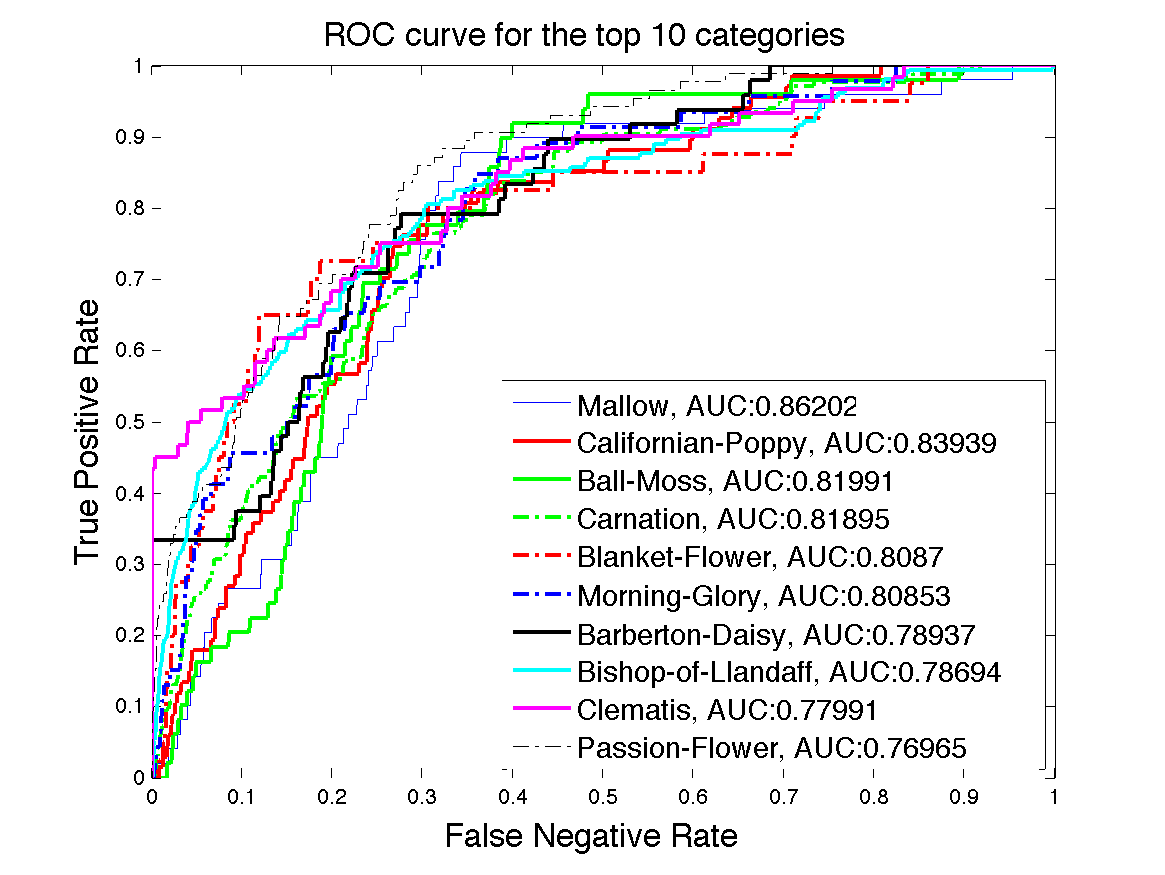
\includegraphics[width=1.00\linewidth,height=.66\linewidth]{figroc.eps}
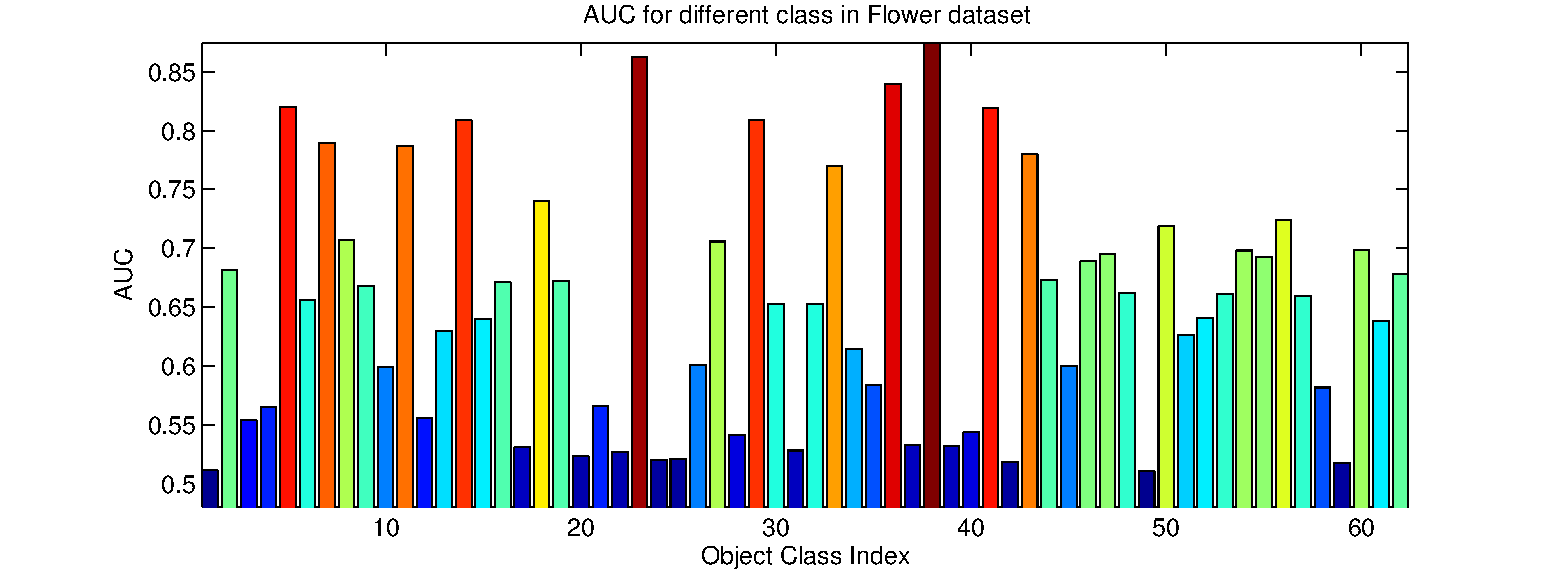
\includegraphics[width=1.00\linewidth,height=.34\linewidth]{fig1auc.eps}
%\caption{ROC-curves for the top 10 classifiers in Flower dataset}
%\vspace{-2mm}
\caption{Kernel: AUC of the 62 unseen classifiers the flower data-sets over three different splits (bottom part) and their Top 10 ROC-curves (top part)}
%\vspace{-2mm}
\label{F:AUCstop10}
\end{figure}








\begin{comment}
\begin{figure}[h!]
\centering
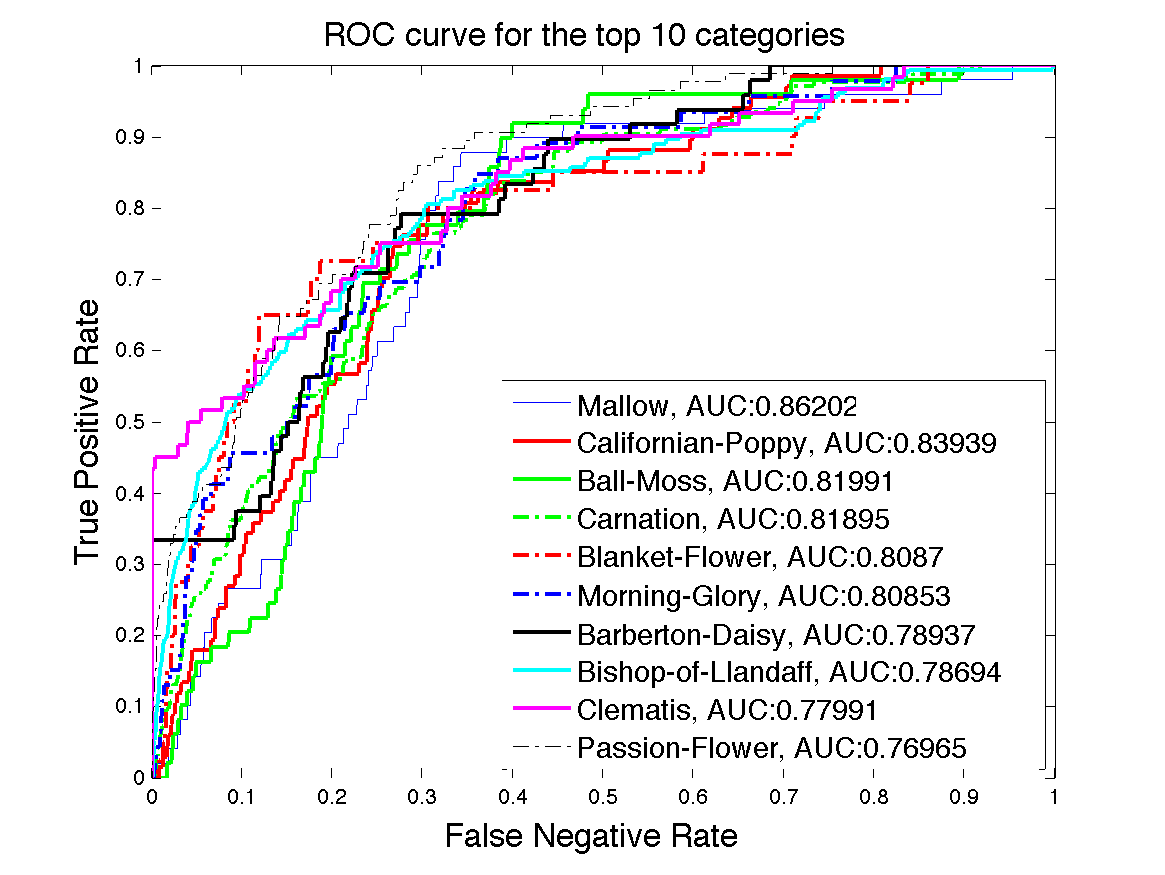
\includegraphics[width=0.7\linewidth,height=.50\linewidth]{figroc.eps}
\caption{ROC-curves for the top 10 classifiers in Flower dataset}
\label{F:top10}
\end{figure}



\begin{figure}[h!]
\centering
 \hspace*{-12mm}%
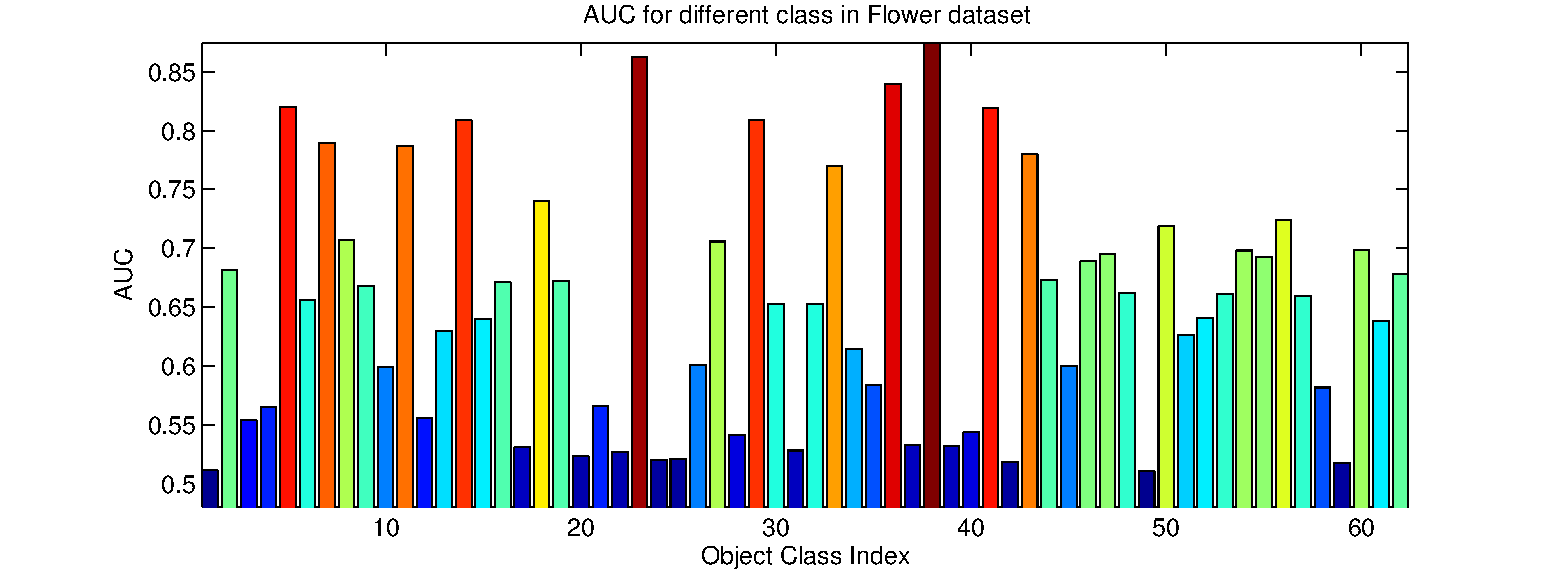
\includegraphics[width=1.0\linewidth,height=.30\linewidth]{fig1auc.eps}
%\vspace{-15pt}
\caption{Kernel: AUC of the 62 unseen classifiers the flower data-sets over three different splits}
\label{F:AUCs}
%\vspace{-15pt}
\end{figure}
\end{comment}
\begin{comment}
\begin{table}[ht!]
\caption{Multi-class Accuracy of the Unseen classes (MAU)  on three seen/unseen splits - Flower Dataset and a seen/unseen split on Birds dataset}
\vspace{-3mm}
\label{tbl:flowerbirdsmau}
  \centering
  \scalebox{0.6}
  {
\begin{tabular}{|c|c|c|c|c|}
\hline 
  & MAU-Flower & improvement & MAU-Birds& improvement \\ 
  \hline 
{SVM-DT kernel-rbf }& \textbf{9.1 (+/-  2.77) \%} & & \textbf{3.4  \%}   &  \\ 
\hline 
{DT kernel-rbf }& \textbf{6.64 (+/-  4.1) \%} & 37.93 \%  & \textbf{2.95  \%} & 15.25 \% \\ 
\hline 
Linear Classifier \ignore{ Prediction} & 5.93  (+/-  1.48)\% & 54.36 \%  & 2.62 \% & 29.77 \% \\ 
\hline 
DT-linear\ignore{~\cite{Hoseini13,da11}} & 5.79 (+/-  2.59)\% & 58.46 \%  &  2.47 \% & 37.65 \%  \\ 
\hline 
\end{tabular} 
}
\end{table}

\begin{table}[ht!]
\caption{Average AUC of the Unseen classes on three  seen/unseen  splits on Flower dataset and a seen/unseen split on Birds dataset }
\label{tbl:flowerbirdsauc}
  \centering
  \scalebox{0.6}
 {
\begin{tabular}{|c|c|c|c|c|}
\hline 
 & AUC-Flower & improvement & AUC-Birds & improvement\\ 
\hline 
{SVM-DT kernel-rbf }& {0.653 (+/-  0.009) } &   &   0.61  &   \\ 
\hline 
{DT kernel-rbf }& {0.623 (+/-  0.01) \%} & 4.7 \% &  0.57  & 7.02 \%  \\ 
\hline 
Linear Classifier \ignore{Prediction} & 0.658 (+/-  0.034) & - 0.7 \% & 0.62  & -1.61\%  \\ 
\hline 
DT-linear\ignore{~\cite{Hoseini13,da11}} &0.644 (+/-  0.008) &  1.28 \% & 0.56  & 8.93\%  \\ 
\hline 
\end{tabular} 
}
\end{table}
\end{comment}


\begin{comment}
\begin{table*}[ht!]
\caption{Multi-class Accuracy of the Unseen classes (MAU)  on a seen-unseen split-Birds Dataset (MKL)}
\label{tbl:birdsmkl}
  \centering
\begin{tabular}{|c|c|c|}
\hline 
& MAU & improvement \\ 
\hline 
{SVM-DT kernel-rbf (text) - mkl (visual) }& \textbf{4.10  \%} &   \\ 
\hline 
Linear Classifier Prediction & 2.74 \% & 49.6 \% \\ 
\hline 
\end{tabular} 
\end{table*}

\begin{table*}[ht!]
\caption{Multi-class Accuracy of the Unseen classes (MAU)  on a seen-unseen split-Birds Dataset (Attributes)}
\label{tbl:birds3}
\centering
\begin{tabular}{|c|c|c|}
\hline 
 & MAU & improvement \\ 
\hline 
{SVM-DT kernel-rbf }& \textbf{5.6  \%} &   \\ 
\hline 
{DT kernel-rbf }& {4.03 \%} &  32.7 \% \\ 
\hline 
Lampert DAP  \ignore{\cite{Lampert09}} & 4.8  \% & 16.6 \% \\ 
\hline 
\end{tabular} 
\end{table*}
\end{comment}

\begin{comment}
\begin{figure*}
  \begin{minipage}[b]{0.25\linewidth}
    \centering
     \captionof{table}{Kernel: MAU on a seen-unseen split-Birds Dataset (MKL)}
\label{tbl:birdsmkl}
    \scalebox{0.6}
  {
\begin{tabular}{|c|c|c|}
\hline 
& MAU & improvement \\ 
\hline 
{SVM-DT kernel-rbf (text)}& \textbf{4.10  \%} &   \\ 
\hline 
Linear Classifier \ignore{Prediction} & 2.74 \% & 49.6 \% \\ 
\hline 
\end{tabular} }
 \vspace{6mm}
\end{minipage}
   \begin{minipage}{0.01\linewidth}$\,$\end{minipage}
 \begin{minipage}[b]{0.25\linewidth} 
     \centering
  \captionof{table}{Kernel: MAU on a seen-unseen split-Birds Dataset (Attributes)} 
\label{tbl:birds3}
    \scalebox{0.6}
  {
\begin{tabular}{|c|c|c|}
\hline 
 & MAU & improvement \\ 
\hline 
{SVM-DT kernel-rbf }& \textbf{5.6  \%} &   \\ 
\hline 
{DT kernel-rbf }& {4.03 \%} &  32.7 \% \\ 
\hline 
Lampert DAP\ignore{  \cite{Lampert09}} & 4.8  \% & 16.6 \% \\ 
\hline 
\end{tabular} }
\vspace{6mm}
\end{minipage}      
   \begin{minipage}{0.01\linewidth}$\,$\end{minipage} \begin{minipage}[b]{0.45\linewidth}
   \hspace{-5.8mm}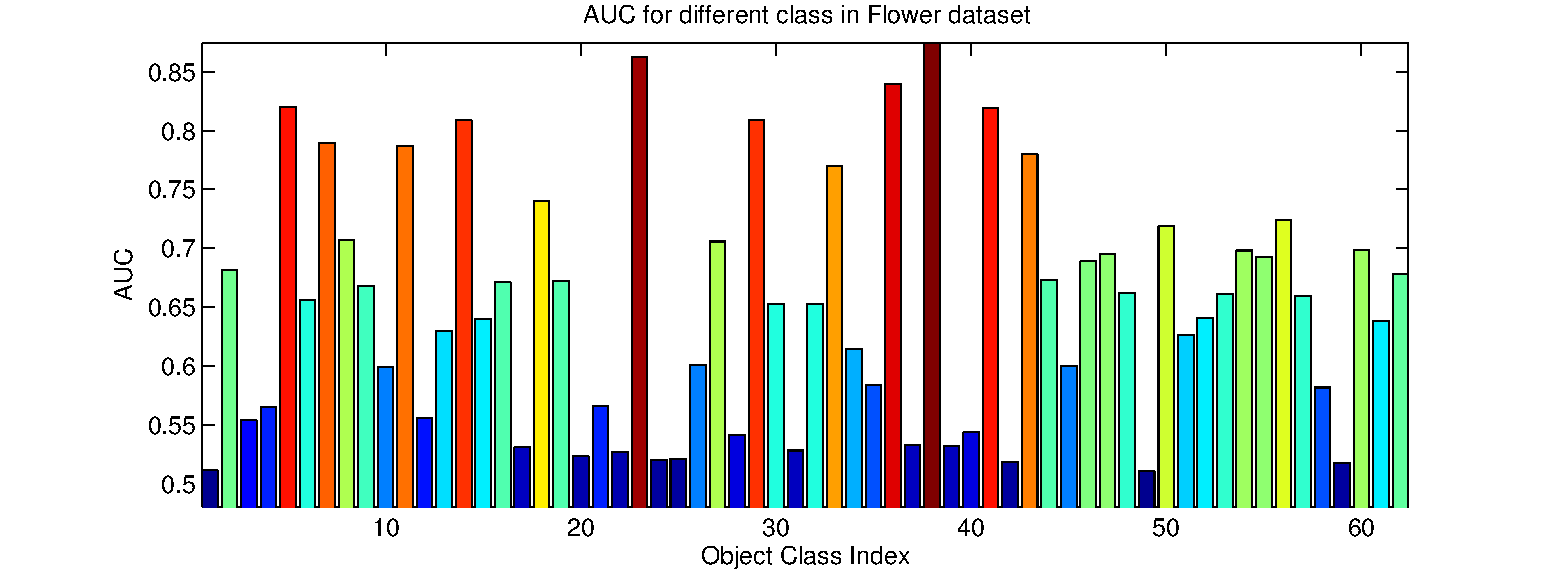
\includegraphics[width=0.6\linewidth,height=.150\linewidth]{fig1auc.eps}
\caption{Kernel: AUC of the 62 unseen classifiers the flower data-sets over three different splits}
\label{F:AUCs}
 \end{minipage}%
\end{figure*}
\end{comment}



\begin{comment}
% This is the good table
\begin{figure*}
  \begin{minipage}[b]{0.25\linewidth}
    \centering
     \captionof{table}{Kernel: MAU on a seen-unseen split-Birds Dataset (MKL)}
\label{tbl:birdsmkl}
    \scalebox{0.55}
  {
\begin{tabular}{|c|c|c|}
\hline 
& MAU & improvement \\ 
\hline 
{SVM-DT kernel-rbf (text)}& \textbf{4.10  \%} &   \\ 
\hline 
Linear Classifier \ignore{Prediction} & 2.74 \% & 49.6 \% \\ 
\hline 
\end{tabular} }
  \centering
   \vspace{2mm}
  \captionof{table}{Kernel: MAU on a seen-unseen split-Birds Dataset (Attributes)} 
\label{tbl:birds3}
    \scalebox{0.6}
  {
\begin{tabular}{|c|c|c|}
\hline 
 & MAU & improvement \\ 
\hline 
{SVM-DT kernel-rbf }& \textbf{5.6  \%} &   \\ 
\hline 
{DT kernel-rbf }& {4.03 \%} &  32.7 \% \\ 
\hline 
Lampert DAP\ignore{  \cite{Lampert09}} & 4.8  \% & 16.6 \% \\ 
\hline 
\end{tabular}}
 \scalebox{0.6}
  {
\begin{tabular}{|c|c|c|}
\hline 
 & Recall & improvement \\ 
\hline 
{SVM-DT kernel-rbf }& \textbf{76.7  \%} &   \\ 
\hline 
Lampert DAP  \ignore{\cite{Lampert09}} & 68.1  \% & 12.6 \% \\ 
\hline 
\end{tabular}
 }
         \vspace{6mm}
\end{minipage}
 \begin{minipage}[b]{0.01\linewidth}$\,$\end{minipage}
  \begin{minipage}[b]{0.27\linewidth}
  \centering
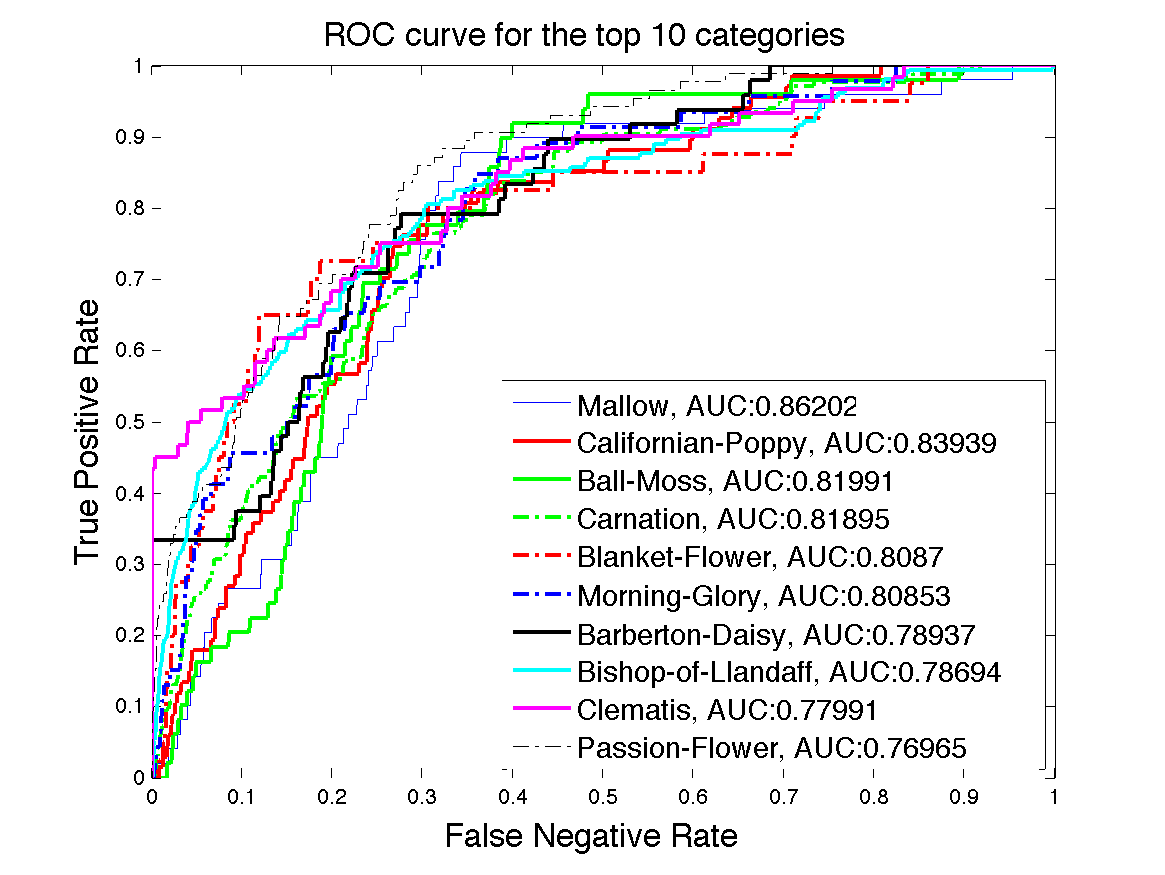
\includegraphics[width=1.0\linewidth,height=.72\linewidth]{figroc.eps}
\caption{ROC-curves for the top 10 classifiers in Flower dataset}
\label{F:top10}
  \end{minipage}%
   \begin{minipage}{0.01\linewidth}$\,$\end{minipage} \begin{minipage}[b]{0.25\linewidth}
   \hspace{-6.8mm}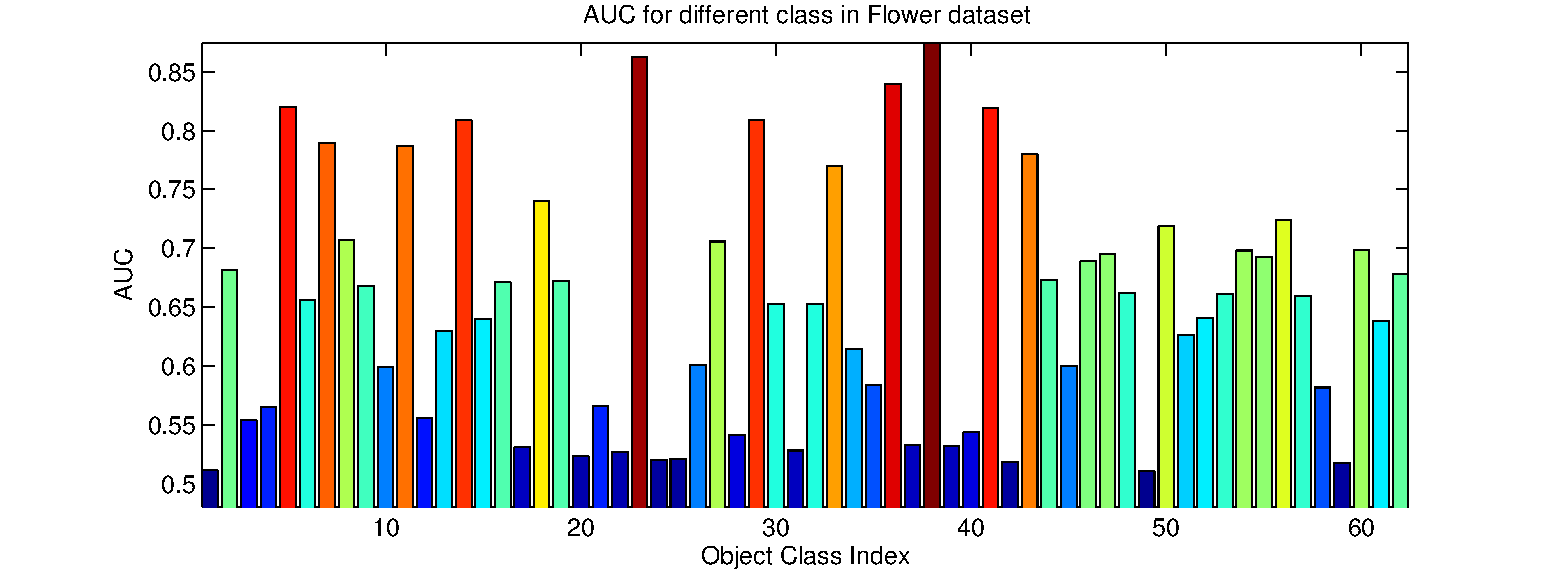
\includegraphics[width=1.15\linewidth,height=.40\linewidth]{fig1auc.eps}
\caption{Kernel: AUC of the 62 unseen classifiers the flower data-sets over three different splits}
\label{F:AUCs}
 \end{minipage}%
\end{figure*}
%\vspace{-10mm}

 \end{comment}

%\textit{Conclusion on textual features as $\mathcal{E}$ space: }
 




 
%\vspace{-5mm}
\begin{comment}
\begin{table}[h!]
\caption{Average AUC of the Unseen classes on three three seen/unseen  splits - Flower Dataset}
\label{tbl:flowerauc}
  \centering
\begin{tabular}{|c|c|c|}
\hline 
 & AUC & improvement \\ 
\hline 
{SVM-DT kernel-rbf }& {0.653 (+/-  0.009) } &   \\ 
\hline 
{DT kernel-rbf }& {0.623 (+/-  0.01) \%} & 4.7 \% \\ 
\hline 
Linear Classifier Prediction & 0.658 (+/-  0.034) & - 0.7 \% \\ 
\hline 
Domain Transfer~\cite{Hoseini13,da11} &0.644 (+/-  0.008) &  1.28 \%\\ 
\hline 
\end{tabular} 
\end{table}


\begin{table}[htbp]
  \centering
  \caption{Average AUC of the Unseen classes on a seen/unseen  split - Birds Dataset }
  \label{tbl:birdsauc}
    \begin{tabular}{|c|c|c|}
  \hline 
 & AUC & improvement \\ \hline 
    SVM-DT kernel-rbf & 0.61  &  \\\hline 
    DT-kernel-rbf & 0.57  & 7.02 \% \\ \hline 
    Linear Classifier Prediction & 0.62  & -1.61\% \\ 
    \hline 
    Domain Transfer~\cite{Hoseini13,da11}  & 0.56  & 8.93\% \\
    \hline 
    \end{tabular}
  \label{tab:addlabel}
\end{table}
\end{comment}



%\vspace{-10mm}
\begin{comment}

\begin{table*}[ht!]
\caption{Multi-class Accuracy of the Unseen classes (MAU)  on a seen-unseen split-Birds Dataset}
\label{tbl:birds}
  \centering
\begin{tabular}{|c|c|c|}
\hline 
& accuracy & improvement \\ 
\hline 
{SVM-DT kernel-rbf }& \textbf{3.4  \%} &   \\ 
\hline 
{DT kernel-rbf }& {2.95  \%} & 15.25 \% \\ 
\hline 
Linear Classifier Prediction& 2.62 \% & 29.77 \% \\ 
\hline 
Domain Transfer~\cite{Hoseini13,da11} & 2.47 \% & 37.65 \% \\ 
\hline 
\end{tabular} 
\end{table*}
\begin{table*}[ht!]
\caption{Multi-class Accuracy of the Unseen classes (MAU)  on three seen/unseen splits - Flower Dataset}
\label{tbl:flower}
  \centering
\begin{tabular}{|c|c|c|}
\hline 
  & accuracy & improvement \\ 
  \hline 
{SVM-DT kernel-rbf }& \textbf{9.1 (+/-  2.77) \%} &   \\ 
\hline 
{DT kernel-rbf }& \textbf{6.64 (+/-  4.1) \%} & 37.93 \% \\ 
\hline 
Linear Classifier Prediction & 5.93  (+/-  1.48)\% & 54.36 \% \\ 
\hline 
Domain Transfer~\cite{Hoseini13,da11} & 5.79 (+/-  2.59)\% & 58.46 \% \\ 
\hline 
\end{tabular} 
\end{table*}
\end{comment}

\subsubsection{Multiple Kernel Learning (MKL) Experiment}

This experiment shows the added value of  proposing a kernelized zero-shot learning approach. We conducted an experiment where the final kernel on the visual domain is produced by Multiple Kernel Learning \cite{MKKLAlgs11}. For the visual domain, we extracted kernel descriptors for Birds dataset. Kernel descriptors provide a principled way to turn any pixel attribute to patch-level features, and are able to generate rich features from various recognition cues. We specifically used four types of kernels introduced by~\cite{bo_nips10} as follows: \textit{Gradient Match Kernels} that captures image variation based on predefined kernels on image gradients. \textit{Color Match Kernel} that describes patch appearance using two kernels on top of RGB and normalized RGB for regular images and intensity for grey images. These kernels capture image variation and visual apperances. For modeling the local shape, \textit{Local Binary Pattern} kernels have been applied. We computed these kernel descriptors on local image patches with fixed size 16 x 16 sampled densely over a grid with step size 8 in a spatial pyramid setting with four layers. The dense features are vectorized using codebooks of size 1000. This process ended up with a 120,000 dimensional feature for each image (30,000 for each type). Having extracted the four types of descriptors, we compute an rbf kernel matrix for each type separately. We learn the bandwidth parameters for each rbf kernel by cross validation on the seen classes. Then, we generate a new kernel \small$k_{mkl}(d, d') = \sum_{i=1}^4 w_i k_i(d, d')$\normalsize, such that $w_i$ is a weight assigned to each kernel. We learn these weights by applying Bucak's Multiple Kernel Learning algorithm \cite{nips10_Bucak}. Then, we applied our approach where the MKL-kernel is used in the visual domain and rbf kernel in the text domain similar to the previous experiments.



 To compare the kernel prediction approach to the linear prediction approach (formulation (E)) under this setting,  we concatenated  all kernel descriptors to end up with  120,000 dimensional feature vector in the visual domain. As highlighted in  the kernel approach section, the linear prediction approach solves a quadratic program of \small$N+d_v+1\,$\normalsize variables for each unseen class.   Due to the large dimensionality of data  (\small$d_v = 120,000$\normalsize), this is not tractable. To make this setting applicable, we reduced the dimensionality of the feature vector into $4000$ using PCA\ignore{ to make it feasible to compute the performance}. This highlights the benefit of our approach since our quadratic program does not depend on the dimensionality of the data. Table ~\ref{tbl:birdsmkl} shows MAU for the kernel prediction approaches under this setting against  linear prediction. The results show the benefits of having a kernel prediction for zero shot learning where kernel methods to construct an arbitrary kernel that  improves the performance.

\subsection{Multiple Representation Experiment and  Distributional Semantic(DS) Kernel}
\label{sec64}

The aim of this experiment is to show that the kernel approach perform on different representations of text $\mathcal{T}$ and visual domains $\mathcal{V}$. In this experiment, we extracted Convolutional Neureal Network(CNN) image features for the Visual domain. We used caffe~\cite{jia2014caffe} implementation of~\cite{imagenetnips12}. Then, we extracted the sixth activation feature of the CNN (FC6) since we found it works the best on the standard classification setting. We found this consistent with the results of~\cite{donahue2014decaf} over different CNN layers. While using  TFIDF feature of text description and CNN features for images, we achieved 2.65\% for the linear version and 4.2\% for the rbf kernel on both text and images. We further improved the performance to 5.35\% by using our proposed Distributional Semantic (DS) kernel in the text domain and rbf kernel for images. In this DS experiment, we used the  distributional semantic model by~\cite{mikolov2013distributed} trained on  GoogleNews corpus (100 billion words)  resulting in a vocabulary of size 3 million words, and word vectors of $K=300$ dimensions. This experiment shows both the value of having a kernel version and also the value of the proposed kernel in our setting. We also applied the zero shot learning approach in~\cite{norouzi2014zero} which performs worse in our settings; see Table~\ref{tbl:birdscnn}. 



\subsubsection{Attributes Experiment}

We emphasis that our  goal from this experiment is not attribute prediction. However, it was interesting for us to see the behavior of our method where $\mathcal{T}$ space is defined from attributes instead of text. In contrast to attribute-based models, which fully utilize attribute information to build attribute classifiers, we do not learn attribute classifiers. In this experiment, our method  uses only the first moment of information of the attributes (i.e. the average attribute vector). We decided to compare to an attribute-based approach from this perspective. In particular, we applied the  (DAP) attribute-based model~\cite{lampertPAMI13,Lampert09}, widely adopted in many applications (\textit{e.g.,} \cite{liu2013video,rohrbach11cvpr}), to the Birds dataset. 




% in our case will not be easily comparable to attribute-based approaches. We argue that the comparison from this perspective will not be conclusive for the following two reasons. 1) if the comparison is not in our favor, that does not role out the value of our work as a step towards a general approach for predicting classifier without explicit attribute definition  2) If the comparison is in our favor, one might argue better results could have been obtained with better attribute definition/learning. 


For this experiment, we compute the average attributes provided with images for each category, without learning any binary classifiers.  We computed this as  \small$\mathcal{T}\,$\normalsize domain representation for the Birds dataset only, since the Flower dataset does not have attributes. Attribute annotation of Birds dataset is provided in terms of: ``Visibility" and ``Certainty". The first term is $1$ if the attribute is visible and $0$ otherwise. The second term indicates how certain the annotator was about his decision with three levels of ``Certain", ``Guessing" and ``probable". We assigned probability of a visible attribute when the annotator is sure about his decision to $1$ and when he is sure of not seeing the attribute to $0$. All other combination of decisions fall in the range of $(0,1)$. As this attribute annotation is provided for each images, we averaged these scores across all the samples of a class to get a single attribute descriptor for each class, to be consistent with our learning setting. For visual domain, we used classeme features in this experiment (as table~\ref{tbl:flowerbirdsmauauc} experiment )\ignore{(as in section ~\ref{exp1} )}. 




%In contrast to attribute-based models, which fully utilize attribute information to build attribute classifiers, our approach do not learn attribute classifiers since we do. \ignore{Also in our approach  attributes are only defined at the class level. In that sense,} Our method also uses only the first moment of information of the attributes (i.e. the average attribute vector). We decided to compare to an attribute-based approach from this perspective. In particular, we applied the  (DAP) attribute-based model \cite{Lampert09,lampertPAMI13}, widely adopted in many applications (\textit{e.g.} \cite{rohrbach11cvpr}), to the Birds dataset.

   
\begin{table}
\centering
 \caption{Kernel: Recall and MAU on a seen-unseen split-Birds Dataset (Attributes)} 
\label{tbl:birds3}
 \vspace{-1mm}
\scalebox{1.0}
  {
\begin{tabular}{|c|c|c|}
\hline 
 & Recall & improvement \\ 
\hline 
{SVM-DT kernel-rbf }& \textbf{76.7  \%} &   \\ 
\hline 
Lampert DAP  {\cite{Lampert09}} & 68.1  \% & 12.6 \% \\ 
\hline 
\end{tabular}
 }

    \scalebox{1.0}
  {
\begin{tabular}{|c|c|c|}
\hline 
 & MAU & improvement \\ 
\hline 
{SVM-DT kernel-rbf }& \textbf{5.6  \%} &   \\ 
\hline 
{DT kernel-rbf }& {4.03 \%} &  32.7 \% \\ 
\hline 
Lampert DAP {  \cite{Lampert09}} & 4.8  \% & 16.6 \% \\ 
\hline 
\end{tabular}}

 \vspace{-2mm}
\end{table}

An interesting result is that our approach achieved $5.6\%$  MAU ($224\%$ the random guess performance); see Table ~\ref{tbl:birds3}. In contrast, we get $4.8\%$ multiclass accuracy using  DAP approach~\cite{lampertPAMI13}. In this setting, we also measured the $N_{sc}$ to $ N_{sc}+1$ average recall. We found the recall measure is $76.7\%$ for our SVM-DT-kernel, while it is $68.1\%$ on  the DAP approach, which reflects better true positive rate (positive class is the unseen one). We find these results interesting, since we achieved it without learning any attribute classifiers, as in~\cite{lampertPAMI13}. When comparing the results  of our approach using attributes (Table~\ref{tbl:birds3}) vs. textual description (Table~\ref{tbl:flowerbirdsmauauc})\footnote{We are refering to the experiment that uses classeme as visual features to have a consistent comparison to here} as the $\mathcal{T}$ space used for prediction, it is clear that the attribute features gives better prediction. This support our hypothesis that the more meaningful the \small$\mathcal{T}\,$\normalsize domain, the better the performance on \small$\mathcal{V}\,$\normalsize domain. This indicates that if a better textual representation is used, a better performance can be achieved. Attributes are a good semantic representation of a class but it is difficult to  define attributes for an arbitrary class and further measure the confidence of each one. In contrast, it is much easier to find an unstructured  text description for visual class. 


%In this experiment, we compare our approach with an attribute-based approach~\cite{Lampert09} on Birds dataset, for the purpose argued earlier in this section. 
%Table~\ref{tbl:birds3} shows the results of this experiment. 
%An interesting result is that our approach achieved $5.6\%$  MAU ($224\%$ the random guess performance) \ignore{($36.36\%$ of the multiclass accuracy of seen classes (i.e. $15.4\%$))}. In contrast, we get $4.8\%$ multiclass accuracy using  DAP approach~\cite{Lampert09}. In this setting, we also measured the $N_{sc}$ to $ N_{sc}+1$ average recall. We found the recall measure is $76.7\%$ for our SVM-DT-kernel, while it is $68.1\%$ on  the DAP approach, which reflects better true positive rate (positive class is the unseen one). We find these results interesting, since we achieved it without learning any attribute classifiers, as in~\cite{Lampert09}. 
%\vspace{-5mm}
%\vspace{-5mm}

%When comparing the results  of our approach using attributes (Table~\ref{tbl:birds3}) vs. textual description (Table~\ref{tbl:flowerbirdsmauauc})\footnote{We are refering to the experiment that uses classeme as visual features to have a consistent comparison} as $\mathbb{T}$ space, it is clear that the attribute features gives better prediction. This support our hypothesis that the more meaningful the \small$\mathcal{T}\,$\normalsize domain, the better the performance on \small$\mathcal{V}\,$\normalsize domain. This is since, the domain transfer function better captures the correlation between \small$\mathcal{T}\,$\normalsize and \small$\mathcal{V}\,$\normalsize domains in this case. This indicates that if a better textual representation is used, a better performance can be achieved. Attributes are a good semantic representation of a class but it is difficult to  define attributes for an arbitrary class and further measure the confidence of each one. In contrast, it is much easier to find a text description for class. 






